%!TEX root = ../thesis.tex
\chapter{Background}
\label{ch:background}

This thesis uses newly developed approaches from applied topology to study problems in evolutionary biology and genomics.
In this chapter we provide background material on the 
In Section~\ref{bg:bio}
In Section~\ref{bg:tda}
Finally, in Section~\ref{bg:top4bio}

Here we supply sufficient background to motivate our approach.

\section{Biology}
\label{bg:bio}

In this section we present a basic introduction to molecular sequence data: what the data looks like, the processes by which it is generated, and the methods by which it is analyzed.
Particular attention is paid to modes of reticulate evolution.
Exposition for specific applications can be found in their respective individual chapters.

\subsection{Genes and Genomes}
\label{bg:bio:genes}

The information required to express an organism's biological form and function is contained in the genome.
Physically, the genome is manifest as a sequence of nucleotides (DNA), at least one copy of which is packaged inside each cell of an organism.
Abstractly, the genome is represented as a linear sequence of characters defined over the alphabet $\{A,C,G,T\}$.\footnote{The linear representation can be misleading, as many organisms, primarily viruses and bacteria, have circular genomes.}
Contained in this sequence are subsequences representing genes, which code for the protein products that ultimately affect function.
Further embedded in the genome is a complex regulatory pattern of transcription factors controlling the expression of particular genes and directing cellular differentiation and development.

Following the central dogma of biology, DNA is transcribed into RNA, RNA is translated into amino acids, and amino acids are folded into proteins \cite{Crick:1970wb}.
Proteins comprise the functional unit of biology.

Beyond simply coding for function, the genome includes an imprint of the evolutionary history that gave rise to the organism.
By comparing the genomes of multiple organisms, inferences can be drawn about the evolutionary relationships among extant organisms as well as the processes that generated bserved diversity.
The field concerned with exploring these relationships is \emph{comparative genomics}.

\subsection{Evolutionary Processes}
\label{bg:bio:evolution}

Evolution describes the gradual change in phenotypes arising from random variation and subject to natural selection.
The processes giving rise to diversity can be classified into two types: clonal and reticulate.

\subsubsection{Clonal Evolution}
\label{bg:bio:evolution:clonal}

Clonal evolution, or vertical evolution, is a process of self-reproduction whereby genetic material is transferred directly from parent to offspring.
Population diversity is generated by stochastic mutation and maintained over multiple generations by random drift.

It is clonal evolution that Darwin had in mind when he described the idea of descent with modification, whereby a parent passes genomic information to an offspring subject to random drift.
Importantly, because there is always a direct parent--offspring relationship, clonal evolution will be consistent with a phylogenetic tree model.

\subsubsection{Reticulate Evolution}
\label{bg:bio:evolution:reticulate}

Reticulate evolution, or horizontal evolution, refers to exchange or acquisition of genetic material via processes that do not reflect a direct parent--offspring relationship.
As we will see, these processes can make inferences about historical evolutionary relationships difficult.
Different types reticulate processes occur in different types of organisms (summarized in Table \ref{table:reticulation_processes}).

Viruses replicate by infecting a host cell and then using the host cell machinery and resources to produce multiple copies of viral genetic material.
The genetic material is then packaged into new virus particles which are shed off in order to infect new cells.
Reticulation can occur when two virus particles coinfect the same host cell.
During the replication process, genetic material can be exchanged in one of two ways: \emph{reassortment} or \emph{recombination} (the two processes are contrased in Figure~\ref{fig:viral_reticulation}).
Reassortment occurs in viruses whose genomes are segmented, such as influenza.
Segments are similar to chromosomes, such that a single virus particle will contain a single copy of each segment.
Reassortment occurs when coinfection results in packaging of segments taken from different virus particles.
The result viral progeny will then be a genetic mixture of segments from each parental strain.
Recombination, more common in nonsegmented viruses such as HIV, involves a break-rejoin mechanism during the replication process.
Here, an error in the polymerase during replication can result in an incomplete copy of the genome (a break).
At this point, several cellular processes involved in repair can be recruited to complete the replication process using a homologous region.
If coinfection has occurred, it is possible for these processes to initiate repair using material from a different parental strain.
The outcome will be novel genetic material that includes a crossover from one strain to another.
Break-rejoin crossover is a type of \emph{homologous recombination}.

\begin{figure}
\centering
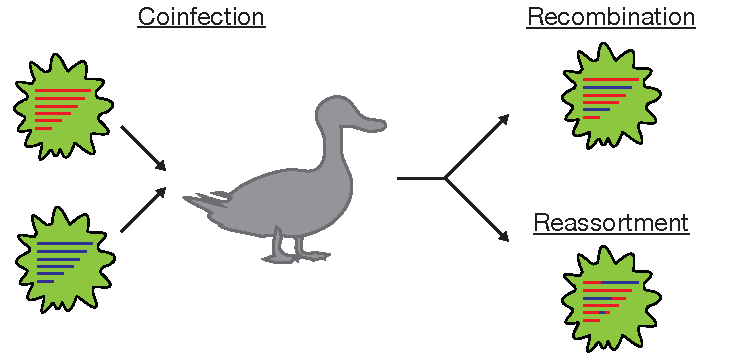
\includegraphics[]{./fig/background/viral_reticulation.pdf}
\caption[Viral recombination and reassortment]{The two modes of viral reticulation. Coinfection of the same host cell can lead to either reassortment, in which whole viral segments are exchanged, or recombination, in which breakpoints can occur within segments. The former process is common in influenza, the latter in HIV. The end result, however, is a novel virus particle which shares genetic information from both parents.}
\label{fig:viral_reticulation}
\end{figure}

In bacteria and other prokaryotes, reticulate evolution can occur when foreign DNA from a donor is acquired by a target organism and integrated into its genome.
Three generic mechanisms have been identified, depending on the route by which foreign DNA is acquired \cite{Ochman:2000dr}:
\begin{enumerate}
\item \emph{Conjugation}. Direct cell-to-cell contact between donor and recipient resulting in transfer of plasmid.
\item \emph{Transformation}. Foreign DNA acquired via uptake from freely circulating DNA in the environment.
\item \emph{Transduction}. Virus-mediated transfer for foreign DNA from an infected donor cell.
\end{enumerate}
A visualization of these three mechanisms is shown in Figure~\ref{fig:bacterial_reticulation}.
Beause these mechanisms can often lead to the acqusition of novel sequences coding for genes not in the recipient organism, reticulate evolution in prokaryotes is often called \emph{horizontal gene transfer} or \emph{lateral gene transfer}.

\begin{figure}
\centering
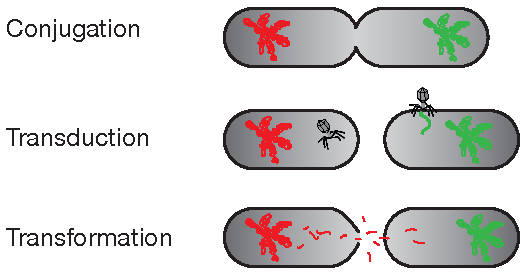
\includegraphics[]{./fig/background/bacterial_reticulation.pdf}
\caption[Three modes of bacterial reticulation]{Three modes of viral reticulation. (1) Conjugation, in which direct cell-to-cell contact results in transfer of genetic material; (2) Transformation, in which foreign DNA is acquired via uptake from freely circulating DNA in the environment; and (3) Transduction, in which exchange of genetic material is mediated by a virus or phage particle.}
\label{fig:bacterial_reticulation}
\end{figure}

In eukaryotes, several reticulate processes have been identified.
We mention two such processes: hybrid speciation and meitotic recombination.
These two processes act at very different scales, but the outcome is the same: a unique offspring with genetic material drawing from both parents.

First, hybrid speciation refers to the cross-breeding of animals or plants of different species.
This mixing of genetic material can lead to the development of a third species with a phenotype distinct from both parents.
Hybrid speciation was originally believed to be a rare occurrence in nature and hybrid offspring to be infertile.
However, recent genomic data has demonstrated that hybrid speciation occurs quite frequently in plants \cite{Arnold:1996,Arnold:2007vq}.
Indeed, Mendel's early experiments in hybridization were themselves an artifically induced form of reticulate evolution.

Second, meiotic recombination refers to a specialized process for generating diversity that occurs in sexually-reproducing polyploid organisms, such as humans, during meiosis.
Meiosis is the process by which a single cell containing $n$ copies of each chromosome results in four distinct cells each with $n/2$ copies of each chromosome.
These special cells are called gametes.
Sexual reproduction consists of the fusion of two gametes during fertilization to form a zygote, which ultimately develops into a viable offspring.
Meiosis is a multistep process consisting of an initial round of DNA replication followed by two rounds of cell division.
Meiotic recombination occurs after the initial round of DNA replication and prior to cell division.
After DNA replication, there are two copies of each homologous chromosome that are joined at a centromere.
The two sets of chromosomes then pair with each other and exchange DNA through physical interactions known as crossovers.\footnote{These crossovers have been shown to not occur randomly, but rather at recombination hotspots regulated by binding motifs for by the PRDM9 protein. \kje{Cite Pablo Paper and a Molly paper}.}
This is another example of homologous recombination and results in new allelic patterns mixing genetic information from both parents.\footnote{Patterns of shared alleles define the concept of \emph{linkage}.}
After crossover occurs, two phases of cellular division result in gametes with $n/2$ copies of each chromosome.

At this point, one might wonder about sexual reproduction -- an offspring can be seen as a hybridization of genetic material donated from both mother and father.
On the one hand, the answer could be yes, particulare because the presence of meiotic recombination involves a shuffling of genomic material such that the chromosome each parent donates is a unique combination of alleles not previously present in the donor organism.
On the other hand, the answer could be no, because both mother and father donte a complete copy of the genome to the offspring.
Each copy can be considered as an independent transfer of genetic information defining both a matrilineal and a patrilineal line of inheritence.
Indeed, researchers in human population genetics generally distinguish between these two cases -- looking at genomic regions that do not recombine they define a matrilinearl common ancestor known as \emph{Mitochondrial Eve} and a patrilineal common ancestor known as \emph{Y-chromosomal Adam}.
Mathematically, the evolutionary relationships of a population of $N$ organisms with ploidy $n$ are often analyzed as a haploid population of size $nN$ with random mating.

\begin{tabularx}{\textwidth}{lll}
\toprule
Organism & Process & Description \\
\midrule
\multirow{2}{*}{Virus} & Reassortment & Exchange of discrete genomic segments \\
                       & Recombination & Intragenomic homologous crossover \\
\midrule
\multirow{3}{*}{Bacteria} & Transformation & Acqusition of foreign DNA in environment \\
                          & Transduction   & Viral-mediated exchange \\
                          & Conjugation    & Cell-to-cell contact and exchange \\
\midrule
\multirow{2}{*}{Eukaryotes} & Meiotic Recombination & Homologous crossover during meiosis \\
                            & Hybrid Speciation         & Fertilization across species boundaries \\
\bottomrule
\label{table:reticulation_processes}
\end{tabularx}

The presence of reticulate processes in a set of organisms can be most clearly identified by comparing phylogenetic relationships built from different genomic segments.
A general practice is to construct the set of \emph{gene trees} which reflect ancestral branching patterns at specific loci.
If a reticulate event has occurred, it implies that the branching patterns of different genes will not agree.
A subfield of comparative genomics is concerned with building \emph{species trees} from sets of gene trees.

However, in the case where there is substantial disagreement among gene trees, the very notion of a species tree may be flawed.
Traditionally, evolutionary biology has concerned itself with characterizing relationships in light of vertical evolution alone.
However, increasing evidence \kje{(what evidence?)} has pointed to the important role played by horizontal evolution, particularly in prokaryotic evolution.
\kje{[Further citations and exposition of Doolittle, Koonin, and Gogarten.]}

\subsection{Mathematical Models of Evolution}
\label{bg:bio:models}

Mathematical population genetics is concerned with properties of populations as they are subject to evolutionary forces over long time scales.
These forces include natural selection, genetic drift, mutation, and recombination.
Historically the input data for population genetics models was comparative studies of allele frequencies across populations.
These studies have primarily been replaced by large-scale genomic surveys which have provided unprecedented insight into ancient population structure and historical migrations.


These models allow two things: 1) simulate genomic data under realistic processes and 2) build statistical models to estimate biological parameters from real data.

\subsubsection{The Wright-Fisher Model}
\label{bg:bio:models:wrightfisher}

The Wright-Fischer model is a forward time simulation of an evolving population.
In the simplest case, the model describes neutral evolution of a constant population size with no structure and constant genome length.
The model proceeds in units of generations.
At each generation, a member of the population is an offspring of a randomly selected ancestor from the previous generation.
This offspring inherits its ancestors genomes, with mutations introduced at some base rate $\mu$.
A member of previous generation with no offspring will be considered extinct.

\subsubsection{The Coalescent Process}
\label{bg:bio:models:coalescent}

The coalescent process is a stochastic model that generates the genealogy of individuals sampled from an evolving population \cite{Wakeley:2009}.
The genealogy is then used to simulate the genetic sequences of the sample.
This model is essential to many methods commonly used in population genetics.
Starting with a present-day sample of $n$ individuals, each individual's lineage is traced backward in time, towards a mutual common ancestor.
Two separate lineages collapse via a coalescence event, representing the sharing of an ancestor by the two lineages.
The stochastic process ends when all lineages of all sampled individuals collapse into a single common ancestor.
In this process, if the total (diploid) population size $N$ is sufficiently large, then the expected time before a coalescence event, in units of $2N$ generations, is approximately exponentially distributed:
\begin{equation}
P(T_{k}=t) \approx \binom{k}{2} e^{-\binom{k}{2} t},
\end{equation}
where $T_k$ is the time that it takes for $k$ individual lineages to collapse into $k-1$ lineages.

After generating a genealogy, the genetic sequences of the sample can be simulated by placing mutations on the individual branches of the lineage.
The number of mutations on each branch is Poisson-distributed with mean $\theta t / 2$, where $t$ is the branch length and $\theta$ is the population-scaled mutation rate.
In this model, the average \emph{genetic distance} between any two sampled individuals, defined by the number of mutations separating them, is $\theta$.

The coalescent with recombination is an extension of this model that allows different genetic loci to have different genealogies.
Looking backward in time, recombination is modeled as a splitting event, occurring at a rate determined by population-scaled recombination rate $\rho$, such that an individual has a different ancestor at different loci.
Evolutionary histories are no longer represented by a tree, but rather by an \emph{ancestral recombination graph}.
Recombination is the component of the model generating nontrivial topology by introducing deviations from a contractibile tree structure, and is the component which we would like to quantify.
Coalescent simulations were performed using \texttt{ms} \cite{Hudson:2002}.

\begin{figure}
\centering
  \subbottom[Wright-Fisher Model]{%
    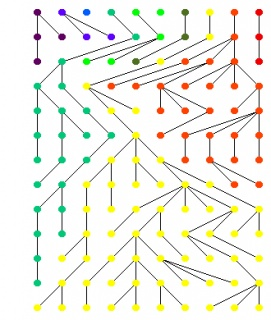
\includegraphics[width=0.3\linewidth]{fig/background/wright-fisher_example.jpg}}
  \subbottom[Coalescent Model]{%
    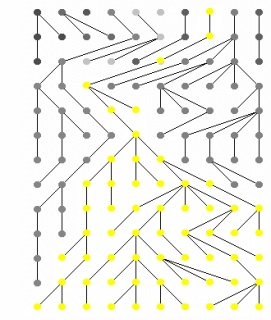
\includegraphics[width=0.3\linewidth]{fig/background/coalescent_example.jpg}}
    \caption{Two models for simulating evolutionary data.}
\end{figure}

% \begin{subfigure}[b]{.1\textwidth}
% 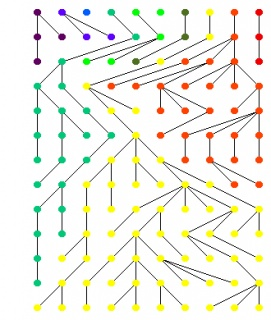
\includegraphics{fig/background/wright-fisher_example.jpg}
% \caption{Wright-Fisher Model}
% \end{subfigure}
% \begin{subfigure}[b]{.1\textwidth}
% 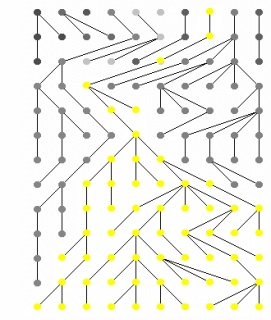
\includegraphics{fig/background/coalescent_example.jpg}
% \caption{Coalescent Process}
% \end{subfigure}
% \end{figure}

\subsubsection{Metrics on Sequences}
\label{bg:bio:models:metrics}

Evolutionary models require a notion of genetic divergence between sequences.
This leads to a discussion of the types of metrics that can be put on sets of sequences.\footnote{Before sequence can be compared, they must first be \emph{aligned}. A sequence alignment arranges the characters in a set of sequences into coluns such that characters sharing evolutionary identity are in the same column. Alignment is necessary because random insertions and deletions can change . The difficulty of performing an alignment will largely depend on the amount of evolutionary divergence in the set of sequences under consideration. Sequence alignment is a well studied topic but largely beyond the scope of this thesis, where we assume sufficient sequence similarity such that alignment can be performed with high confidence.}

The simplest model, and the one most commonly adopted in this thesis, is the Hamming metric, which simply counts the proporation of sites that differ between two aligned sequences.
For example, for two sequence $s_1=ACTTGAC$ and $s_2=AAGTGGC$, $d_{H}(s_1,s_2)=3/7$.
In general, the Hamming metric will underestimate divergences by not accounting for the possibility of back mutations.\footnote{A double mutation of the form $A\rightarrow C\rightarrow A$.}

More biologically motivated models will introduce corrections to account for assumptions about how sequences evolve.
These assumptions include the base frequency of each nucleotide as well as the substitution rates for each type of mutation.
The simplest of these models is the \emph{Jukes-Cantor model}.
This model defines an equal substitution rate $\mu$.
Inverting the probability of an alteration gives the divergence.
The Jukes-Cantor metric is defined as 
\begin{equation}
d_{JC}=-\frac{3}{4}\ln(1-\frac{4}{3}p),
\end{equation}
where $p$ is the proporation of sites that are different.

\subsection{Phylogenetic Methods}
\label{bg:bio:phylo}

A phylogenetic tree is a binary tree in which leaves are associated with particular species or taxa, and the branching pattern of the tree reflects diverging evolutionary relationships.
Branch lengths on the tree are associated with evolutionary divergence between sets of taxa.
Molecular phylogenetics refers to a large collection of methods for inferring branching patterns from aligned molecular sequence data.\footnote{See Felsenstein, \emph{Inferring Phylogenies} for a readable and thorough introduction to the field \cite{Felsenstein:2004ws}.}
In general, the problem of finding an optimal tree associated with sequence data is NP-complete \cite{Foulds:1982fn}, however several approximate methods have been developed.
The primary types of methods include maximum parsimony, distance-matrix methods, maximum likelihood (ML), and Bayesian inference.
Maximum parsimony attempts to find the phylogenetic tree that minimizes the number of evolutionary changes required to explain the observed sequences.
Distance-matrix methods first compute a matrix of pairwise distances between taxa and then find the tree that best approximates these distances.
ML and Bayesian methods use specific models of evolution to assign probability distributions over trees.
In this work we concentrate on distance-matrix methods because of their close connection with the finite metric spaces considered in applied topology.

\subsubsection{Distance-Matrix Methods}
\label{bg:bio:phylo:distance}

Given a set of aligned molecular sequences, distance-matrix methods first compute the pairwise matrix of genetic distances using one of the metrics as described in Section~\ref{bg:bio:models:metrics}.
Then, the binary tree that best approximates those distances is iteratively fit to this data.
This approach to phylogenetic inference were introduced by Cavalli-Sforza and Edwards in 1967 \cite{CavalliSforza:1967th} and Fitch and Margoliash in 1967 \cite{Fitch:1967we}.
The Fitch-Margoliash method uses a weighted least squares approach to tree-fitting, such that larger distances are weighted less, due to higher chances for random error.
Distance-matrix methods are popular for their high speed and scalability as well as high accuracy in most cases.

Currently, the most widely implemented distance-matrix method is neighbor-joining.\footnote{Neighbor joining was introduced by Saitou and Nei in 1987 \cite{Saitou:1987wo}.}
One particular reason neighbor-joining is popular is that under certain conditions, discussed below, it has been shown to exactly recover the correct tree.
The neighbor-joining algorithm is described in Algorithm~\ref{bg:alg:nj}.

\begin{algorithm}
    \KwData{$n \times n$ distance matrix $D$}
    \KwResult{Phylogenetic tree on $n$ leaves}
    \While{rule} {
        Compute $Q$ matrix\;
    }
    \caption{The Neighbor Joining Algorithm. Adapted from Wikipedia entry on Neighbor-Joining.}
    \label{bg:alg:nj}
\end{algorithm}

\subsubsection{Additive Metrics and the Four Point Condition}
\label{bg:bio:phylo:additivity}

Arbitrary distance matrices are unlikely to admit a tree representation.
Those that do are called \emph{additive metrics}, because they can be represented as an additive tree.
Additivity is the property that the distance between any two nodes will be equal to the sum of the branch lengths between them.
A distance matrix admits a tree representation if and only if it is additive.

There is a straight-forward condition that must be satisfied for additivity, known as the \emph{four point condition}.
For a distance matrix to admit a tree representation, 
\begin{equation}
d_{ij} + d_{kl} \leq \max\{d_{ik} + d_{jl} ,  d_{il} + d_{jk} \}
\end{equation}
for any four nodes $\{i,j,k,l\}$.
The condition implies that there is a labeling on the four nodes such that
\begin{equation}
d_{ij} + d_{kl} \leq d_{ik} + d_{jl} =  d_{il} + d_{jk}.
\end{equation}
A visual interpretation of this condition is shown in Figure~\ref{fig:bg:four_point_condition}.

\begin{figure}
\centering
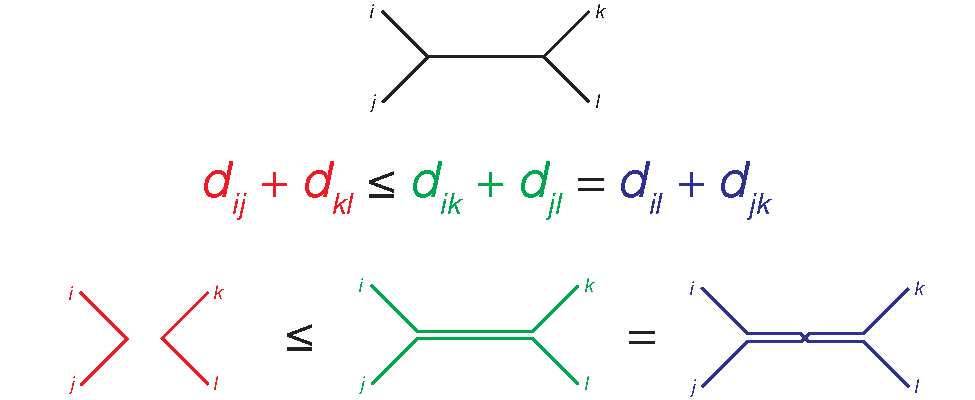
\includegraphics[]{./fig/background/four_point_condition.pdf}
\caption[The four point condition for additivity]{A visual interpretation of the four point condition for additivity. For any four leaves, there exists a labeling $\{i,j,k,l\}$ such that $d_{ij}+d_{kl}\leq d_{ik}+d_{il} = d_{il}+d_{jk}$. Of the three possible ways of arranging the sums of distances, two will involve traversing the internal branch, while one will involve only external branches.}
\label{fig:bg:four_point_condition}
\end{figure}

Sequence data can fail to be additive for several reasons.
First, sequencing error.
Errors can introduce noise into the measured genetic distances.
Second, homoplasy.
A homoplasy occurs when the same mutation is introduced multiple times in a set of organisms.
The presence of homoplasy will underestimate genetic distance between taxa.
Third, reticulate evolution.
As described previously, in cases of reticulate evolution no tree will accurately describe the observed data.

\subsubsection{Number of Tree Topologies}
\label{bg:bio:phylo:topologies}

The number of unrooted bifurcating tree topologies with $L$ leaves is $(2L-5)!!$.\footnote{The double factorial is defined as $n!!=n(n-2)(n-4)\cdots$.}
This can be easily shown using induction.
For $L=3$, we have $\mathcal{T}(3)=1$ and $3$ branches.
To pass to $L=4$, we can add the fourth leaf to any of the $3$ branches, resulting in $3$ different topologies.
For $L=4$, we have $\mathcal{T}(4)=3$.
Every time we add a leaf, we add two branches -- one external and one internal.
For $L=n$, we have $\mathcal{T}(n)=(2n-5)!!$ and $2n-3$ branches.
For $L=n+1$, we can add the new external branch to any of the current $2n-3$ branches.
A rooted tree with $L$ leaves can be considered as an unrooted tree with $L+1$ leaves.
Therefore, the number of rooted bifurcating tree topologies with $L$ leaves is $(2L-3)!!$
As can be seen, the number of tree topologies explodes with the number of leaves.\footnote{It was observed by Walter Fitch that for more than 20 species there are more than Avogadro's number of topologies.}

\subsubsection{The Space of Phylogenetic Trees}
\label{bg:bio:phylo:space}

A phylogenetic tree with $L$ leaves is characterized by its topology and the lengths of each branch.
As shown in the previous section, there are $(2L-5)!!$ possible unrooted topologies.
There are $2L-3$ branches: $L$ external branches and $L-3$ internal branches.
Tree space refers to an abstract construction for representing each possible tree as a point in a geometric space.
Studies of tree space were initiated by Billlera, Holmes, and Vogtmann (BHV) in \cite{Billera:2001tv}.
In that paper, the authors studied rooted trees with zero-length external branches, a space we denote as $\mathrm{BHV}_{L}$.
A geodesic distance was defined between trees of different topology.
This analysis was extended by Zairis \emph{et al.} in \cite{Zairis:2014wa}, in which unrooted trees with non-zero external branches were considered.
The external branches are constrained to sit in the positive open orthan $(\mathbb{R}^{\geq 0})^{L}$.
An evolutionary moduli space is then defined as the product
\begin{equation}
\Sigma_{L} = \mathrm{BHV}_{L-1} \times (\mathbb{R}^{\geq 0})^{L}.
\end{equation}
The tree space construction allows one to define statistics, such as means and variances, on collections of trees in a meaningful way.
An interesting statement that can be made within this framework is that phylogenetics is essentially the projection of real data onto tree space.

We show an exaple of the tree space construction on $L=4$ and $L=5$ leaves in Figure~\ref{fig:bg:tree_space}.
The case of $L=4$ is particularly simple to analyze.
There are three topologies, corresponding to the patterns $((a,b),(c,d))$, $((a,c),(b,d))$, and $((a,d),(b,c))$.
Each topology has a single internal branch.
Attached to each external topology is a space $\mathbb{R}^4$ for the external branches.
The case of $L=5$ also has a relatively simple structure.
There are fifteen possible topologies, each with two internal branches.
The topologies are arranged as a Petersen graph, a common construction in graph theory.
Vertices of the Petersen graph correspond to degenerate points on one of the two internal branches.

\begin{figure}
\centering
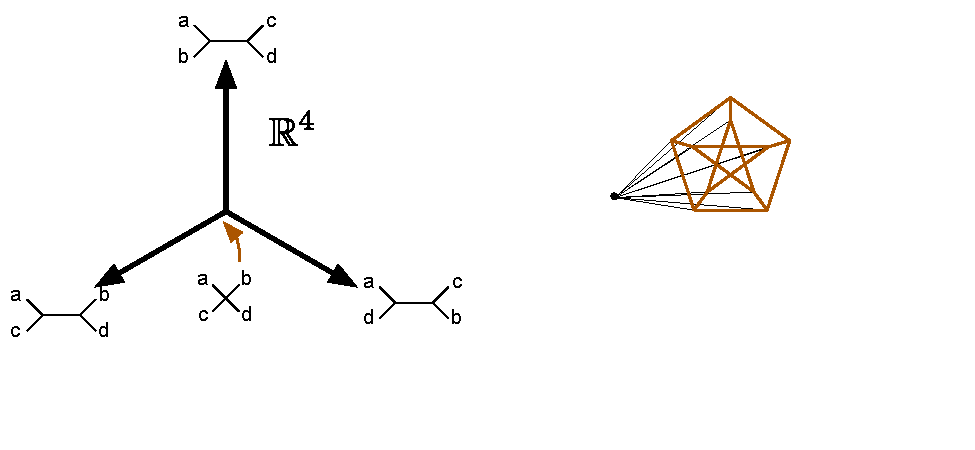
\includegraphics[]{fig/background/tree_space.pdf}
\caption[Tree Space]{Examples of Tree Space. (A) Tree space on 4 leaves. (B) Tree space on 5 leaves.}
\label{fig:bg:tree_space}
\end{figure}

\subsubsection{Phylogenetic Networks}
\label{bg:bio:phylo:networks}

There are several existing methods for representing reticulate evolution.
Most of these methods generalize phylogenetic trees into \emph{phylogenetic networks}, which attempt to reconcile the presence of horizontal evolution in sequence data.
However, most simply present corrections to phylogenetic trees, which can fail in cases where horizontal evolution is pervasive, as in many prokaryote datasets.
Additionally, the resulting networks can be complex and difficult to interpret quantitatively.
This can make it difficult to distinguish between phylogenetic incompatibilities due to noisy sampling and due to true reticulations.
An example of a phylogenetic network using the split network approach is shown in Figure~\ref{fig:bg:split_network}.

\begin{figure}
\centering
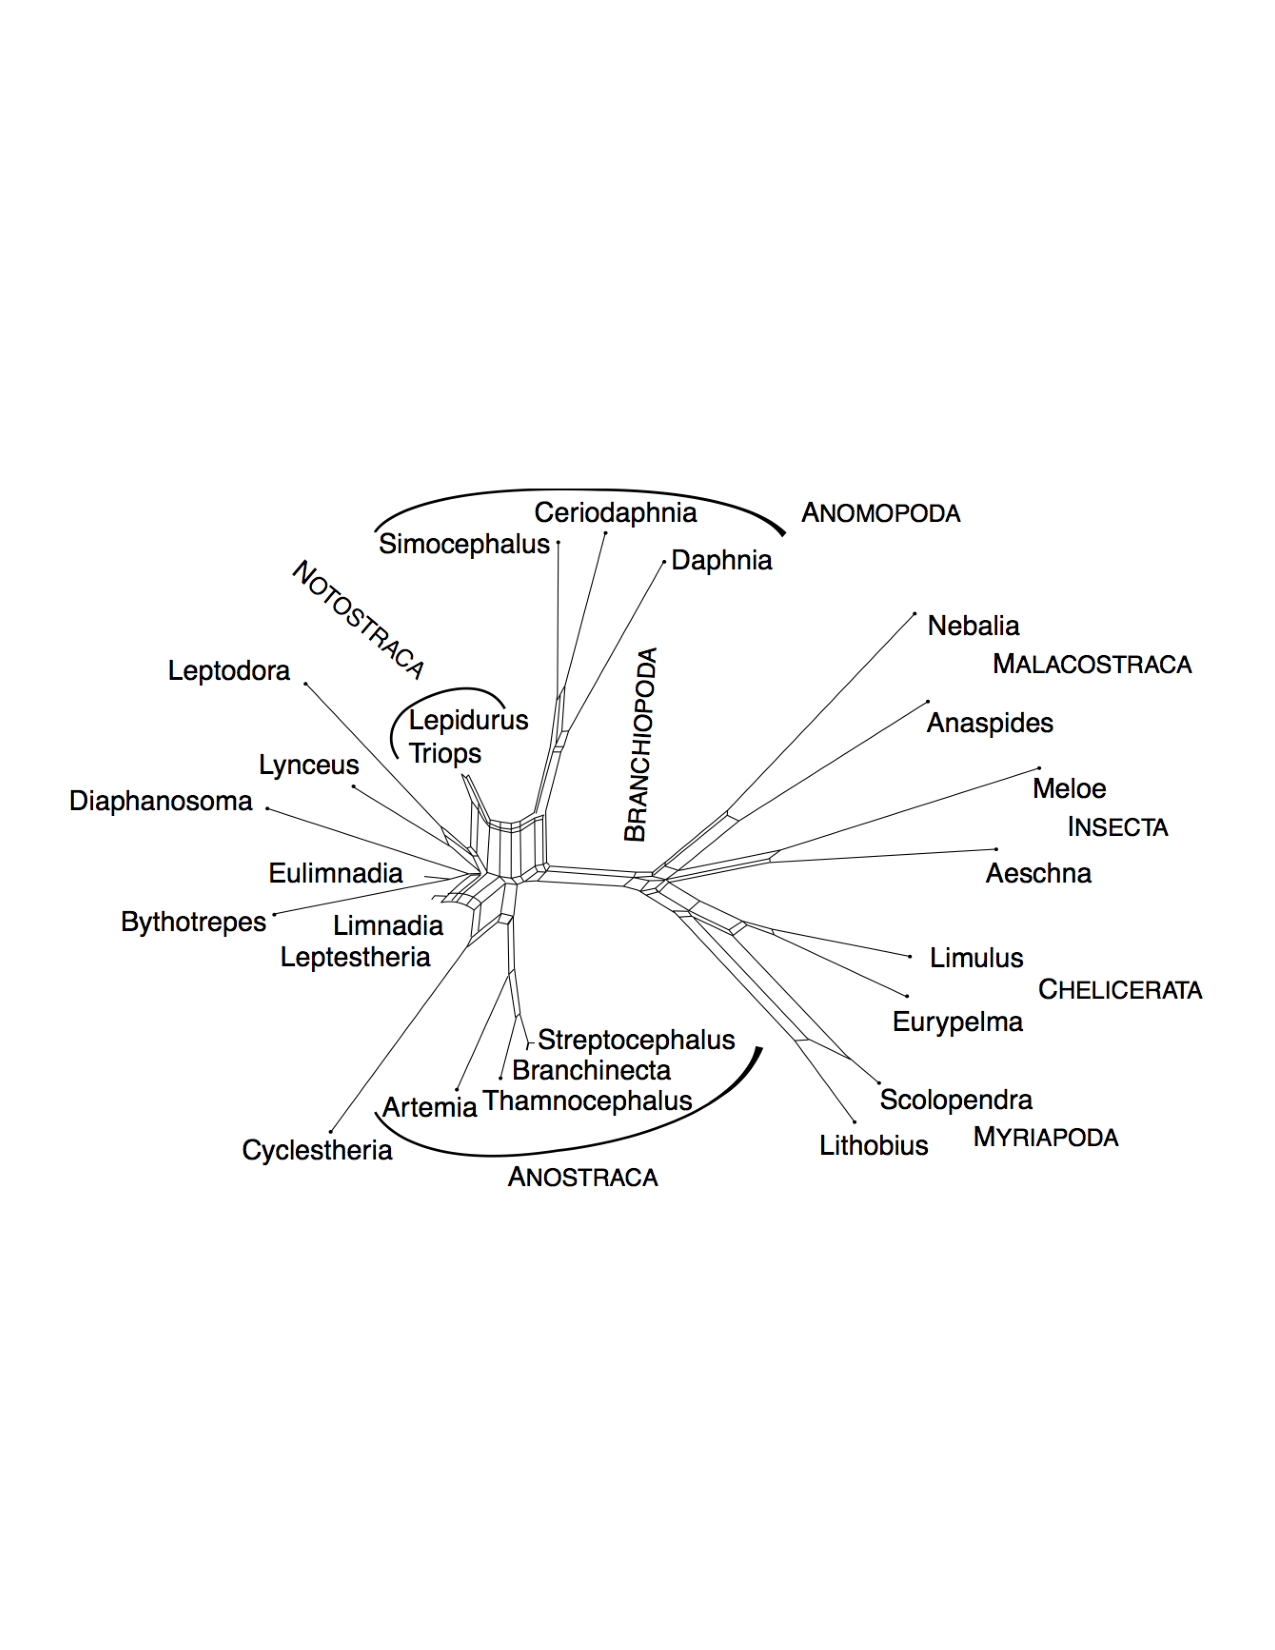
\includegraphics[width=.8\textwidth]{fig/background/split_network.pdf}
\caption[Example of a Splits Network]{Example of a split network of genus Branchiopoda and outgroups. Computed using the Neighbor-Net algorithm. Phylogenetic incompatibilities are represented by conflicting splits. reprinted from BMC Evolutionary Biology 7:147 (2007).}
\label{fig:bg:split_network}
\end{figure}

% NEXT: TDA SECTION. 

\section{Topological Data Analysis}
\label{bg:tda}

Topology is the branch of mathematics that formalizes our intuitive notions of shape.
More concretely, topology provides the methods to characterize the properties of objects and spaces that remain invariant under continuous deformation.
For example, squeezing a circle into an ellipse by compressing along one axis does not change the fact that the object encloses a single loop.
Or, as we saw in the introduction, the coffee mug can be continuously deformed into the donut.
Likewise, if we take a tree and change the lengths of its branches, the tree remains a tree.\footnote{It is important to draw a distinction between the notion of tree topology, in which the branch patterns determines the topology, and global topology, in which all trees are equivalent. While the former is more common in the phylogenetics community, here we consider the latter.}
In each of these examples, while the deformation has substantially altered \emph{local} properties of the space, on a \emph{global} level certain essential characteristics have remained unchanged.
From the perspective of topology, the spaces are considered identical.
The question then is how to formalize our idea of global shape in order to systematically reason about it.

Algebraic topology solves this problem by associating algebraic objects (an integer, for instance) that do not change under continuous deformation.
These objects may capture properties like the number of connected components, the number of loops, and the number of holes in an object, and represent \emph{topological invariants} of a space.
Two spaces can only be deformed into one other if they share the same invariants.
The circle and ellipse are identified as equivalent by the presence of a single loop.
Neither can be deformed into a tree without introducing a cut, which would be a type of discontinuous deformation.
Using these invariants, powerful ideas from abstract algebra can then be used to manipulate and reason about shape.

While topology has traditionally developed through the study of abstract spaces, leading to very rich and beautiful constructions\footnote{For example, see the work of Thurston on low-dimensional topology}, real data does not come in the form of perfect continuous spaces.
Recent effort over the past 15 years has focused on developing methods to apply topology to real world problems in science and engineering.
This work, collectively falling under the heading of \emph{topological data analysis} (TDA), has focused on efficient algorithms for computing topological invariants from finite, noisy data.
TDA now encompasses a wide range of efforts and can now be considered a branch of applied mathematics in its own right.
It has emerged from substantial interdisciplinary effort between mathematicians, computer scientists, and domain experts.

In practice, a typical workflow for applying TDA to real data is as follows.
Data comes in the form of a set of $n$ observations with $p$ attributes, where $p$ is often very large.
The data is assumed to be a finite sample from some more complex space, from which we wish to infer either some sort of global structure or underlying model.
The data is represented as a finite point cloud: a set of $n$ points in $p$ dimensions with an associated notion of distance.
The point cloud is then transformed into a topological space by associating different sets of points with each other.
The associations can be constructed in different ways -- for instance, one of the most common constructions associates points within a certain distance $d$ from one another.
Computational approaches are then used to measure informative topological properties from the space.

In this thesis, we use methods from TDA to study problems in evolutionary biology and genomics.
Our data is typically aligned genomic sequences from sets of related organisms.
If our sequences are each of length $L$, then we can imagine our data as points in an $L$-dimensional sequence space.
A genetic sequence metric, such as the Hamming metric, measures distance.

The two main methods from TDA that we employ are \emph{persistent homology} and \emph{mapper}.
Persistent homology provides a way to efficiently compute the topological invariants of a space across multiple scales, while mapper provides an approach for condensed representation and visualization of high-dimensional data.
In this section, we provide an overview and discussion of these two methods from the perspective of an end-user, treating each method as a pipeline for transforming from raw data to a concise topological summary.
While the mathematical literature on these methods is extremely deep, our goal is to explain things in sufficient detail for a wide audience to grasp the main ideas.
We therefore include a brief introduction of the basic mathematical concepts we employ.
The primary concept we require is \emph{homology}, a particular way in which topological invariants can be assigned to spaces.

The following sections draw on several excellent reviews of TDA, including \cite{Carlsson:2009a}, \cite{Edelsbrunner:2010}, and \cite{Ghrist:2008}.
A more thorough introduction to algebraic topology can be found in \cite{Hatcher:2002ut}.

\subsection{Preliminaries}
\label{bg:tda:math}

As stated above, our data is a set of $n$ points, $S=\{s_1,\ldots,s_n\}$.
Each point is a vector with $p$ features, $s_i=(s_{i1},\ldots,s_{ip})$.
We refer to the collection of points, embedded in a space with an appropriate metric structure, as a point cloud.
We wish to associate a collection of algebraic objects to the point cloud in order to quantify its shape.
To do so, our first step is to construct a topological structure on top of the point cloud, called a \emph{simplicial complex}.
The structure will consist of a set of simplices pieced together in such a way that they approximate the shape of the point cloud in a sensible way.
Shape is then quantified using the notion of \emph{homology}.
This section provides the definitions necessary to understand homology.

\subsubsection{Simplices and Simplicial Complexes}
\label{bg:tda:math:simplices}

The building blocks of our topological structures are simplices.
A \emph{simplex} is something like a point, a line, a triangle, or any higher-dimensional generalization of such.
Formally, a $k$-simplex is a $k$-dimensional polytope which is the convex hull of $k+1$ vertices, as shown in Figure~\ref{fig:bg:simplices}.
A simplex can be represented by its list of vertices, i.e. $\sigma=(s_{1},s_{2},s_{3})$.
An $m$-face of a simplex is the space spanned by the set of $m+1$ vertices, and is itself a simplex.
For example, the $0$-faces and $1$-faces of a simplex are its vertices and edges, respectively.
The $(k-1)$-faces (faces of co-dimension $1$) of a $k$-simplex are called facets.
Facets are represented as $\sigma_{(-i)}$, which implies the facet generated by elimination of the $i$-th vertex.

A \emph{finite simplicial complex} $K$ is built on the vertex set $S$ from simplices glued together in such a way that (1) any face of a simplex in $K$ is also in $K$, and (2) the intersection of any two simplices in $K$ is a face of both simplices.
An example of a simplicial complex is shown in Figure~\ref{fig:bg:simplicial_complex}.

\begin{figure}
\centering
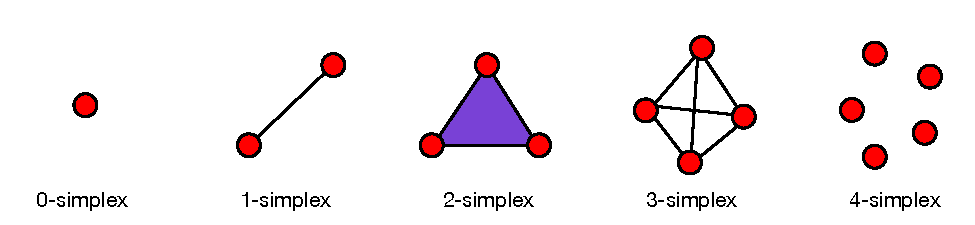
\includegraphics[]{./fig/background/simplices.pdf}
\caption[Simplices: The building blocks of topological complexes]{Simplices are the fundamental building blocks of our topological structures. They can be thought of as triangles generalized to arbitrary dimension. Here we show $k$-simplices for $k=0$ to $k=4$.}
\label{fig:bg:simplices}
\end{figure}

\begin{figure}
\centering
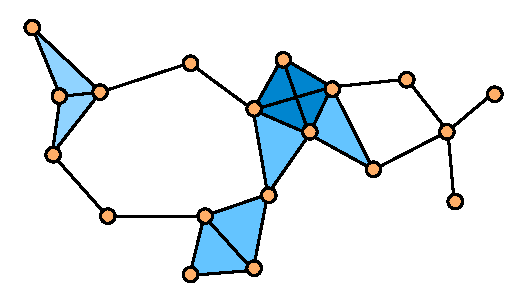
\includegraphics[]{./fig/background/simplicial_complex.pdf}
\caption[Simplicial Complex: A discrete topological space]{A finite simplicial complex is an object built from finite number of simplices glued together in a sensibly nice way.}
\label{fig:bg:simplicial_complex}
\end{figure}

We are interested in combinatorial operations that can be performed on a simplicial complex $K$.
In general, these operations will act on subsets of simplices of fixed dimension $k$.
These subsets are called $k$-\emph{chains}, and can be represented as formal sums $C_{k}=\sum_{j}\alpha_{j}\sigma_{j}$.
The coefficients $\alpha_j$ will be taken to be over $\mathbb{Z}_2$ (i.e. $0$ and $1$).
Two consequences of this choice are (1) $\sigma+\sigma=0$, and (2) we consider simplices without regard to orientation.\footnote{In general, an algebraic topology can be defined with coefficients in arbitrary fields. We use $\mathbb{Z}_2$ for simplicity, efficiency, and because properties, such as torsion, that arise over more complex fields are not expected to be present in the biological data we consider. It is important to keep this in mind, as it was in fact shown that torsion can arise in real data in \cite{Carlsson:2008up}. In that paper, an association was shown between the space of natural images and the Klein bottle.}

An important operator is the boundary operator, $\partial:C_{k}\rightarrow{C_{k-1}}$.
The boundary of a simplex $\sigma$, $\partial_{k}\sigma$, is the sum of its facets.
\begin{equation}
\partial_{k}\sigma = \sum_{i}{\sigma_{(-i)}}
\end{equation}
The boundary of a chain is $\partial C = \sum_{j}\partial\sigma_{j}$.
As a simple example, consider the $2$-simplex $\triangle$ defined by vertices $\triangle=(a,b,c)$.
We have $\partial\triangle = (a,b) + (b,c) + (a,c)$.
Further, we have $\partial\partial\triangle = 2(a) + 2(b) + 2(c) = 0$.
In fact, the property $\partial\partial C = 0$ will hold for any chain $C$.

We can additionally define more refined types of chains.
A \emph{cycle} is a chain with empty boundary, $\partial C=0$.
A \emph{boundary cycle} is a $k$-cycle that is the boundary of a chain in dimension $k+1$.

We can use these definitions to construct various groups on a simplicial complex $K$.
The set of all chains of dimension $k$ forms the chain group $C_{k}$.
The set of all cycles of dimension $k$ forms the cycle group $Z_{k}$.
The set of all boundary cycles of dimension $k$ forms the a group $B_{k}$.
The latter two groups can be understood in terms of the boundary operator $\partial$ acting on $K$.
The group $Z_{k}$ is the kernel of the boundary operator, $Z_{k}=\ker\partial_{k}$.
That is, it is the set of all $k$-chains that are sent to $0$ by the boundary operator.
The group $B_{k}$ is the image of the boundary operator, $B_{k}=\im\partial_{k+1}$.
That is, it is the set of all $k$-chains which are themselves the boundary of $(k+1)$-chains in $K$.
These groups have a particularly simple relationship to one another which is shown in Figure~\ref{fig:bg:chain_complexes}.

% Boundary operator defines a chain complex $C_{*}$:

% \begin{equation}
% \dots \overset{\partial_{n+1}}{\longrightarrow} C_n \overset{\partial_{n}}{\longrightarrow} C_{n-1} \overset{\partial_{n-1}}{\longrightarrow}  ... \overset{\partial_{2}}{\longrightarrow} C_n \overset{\partial_{1}}{\longrightarrow} C_{n-1} \overset{\partial_{0}}{\longrightarrow}  0
% \end{equation}

\begin{figure}
\centering
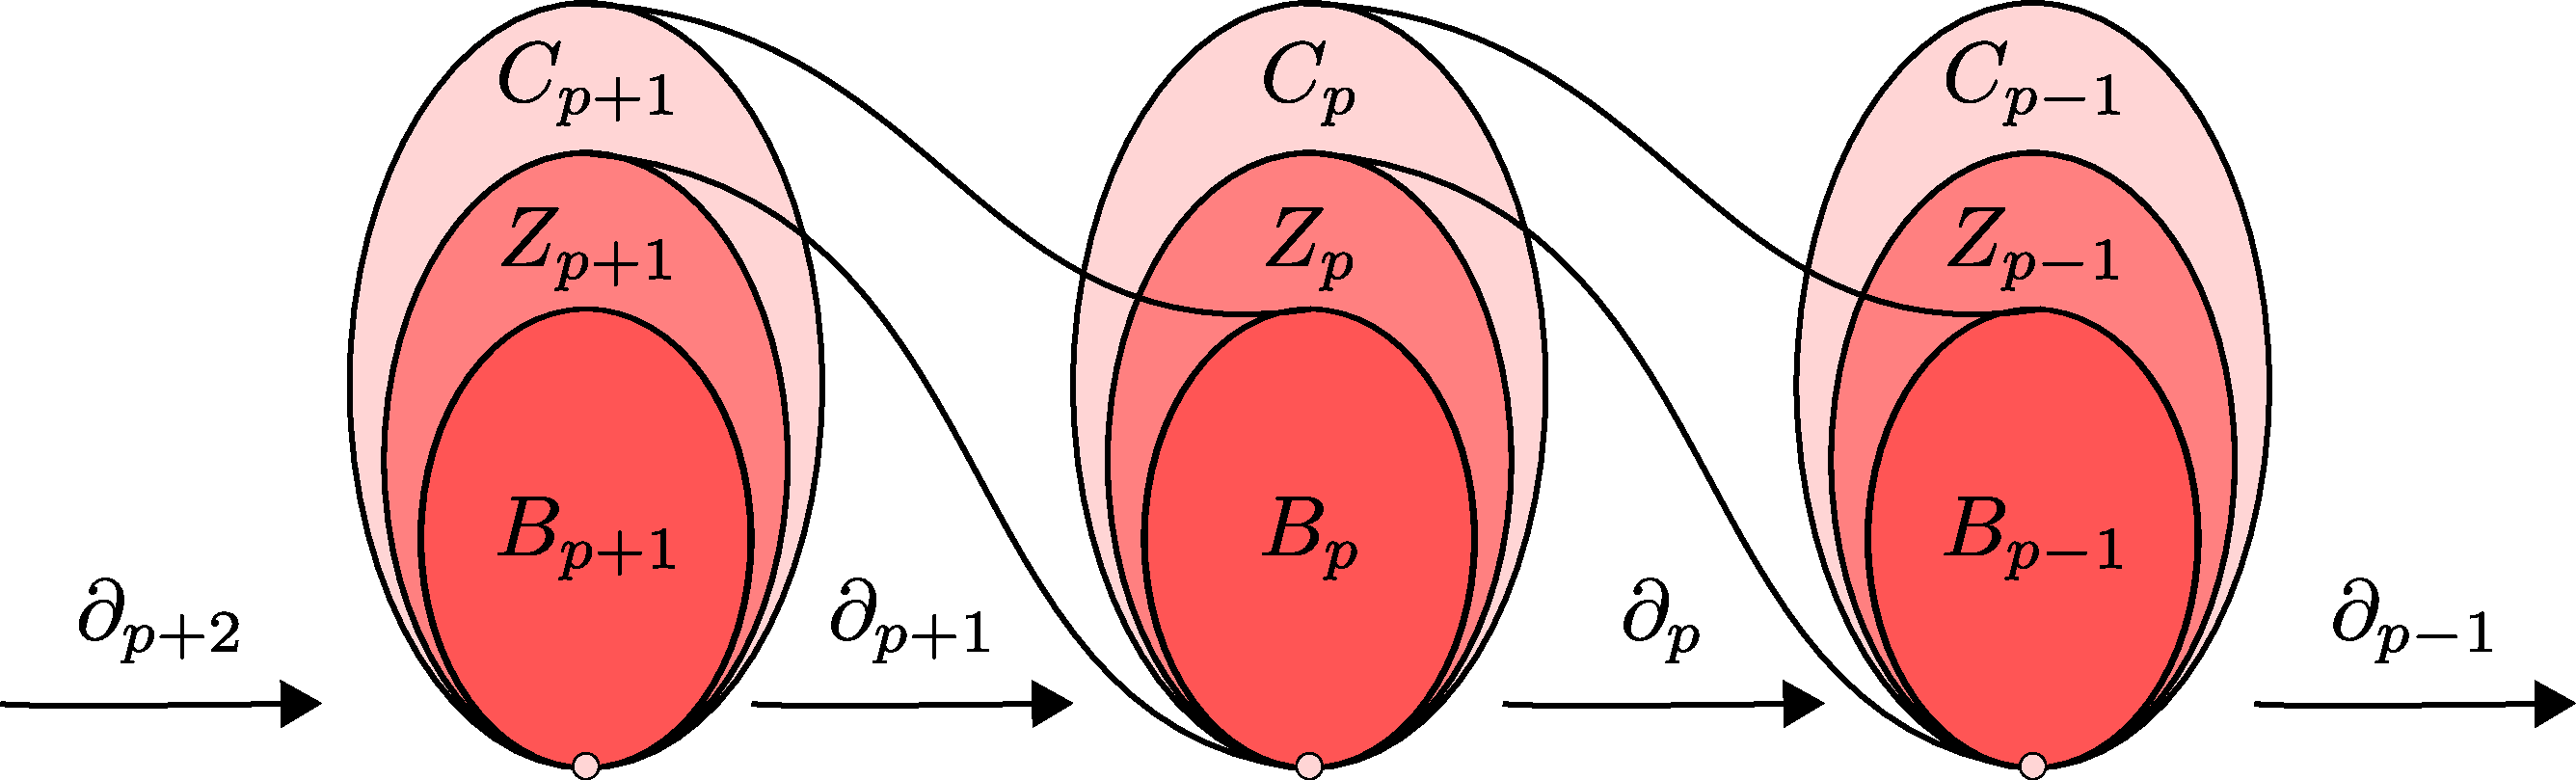
\includegraphics[width=\columnwidth]{./fig/FASY_chain_complexes.pdf}
\caption[Relationship between the chain group, cycle group, and boundary group.]{Relationship between the chain group ($C_p$), cycle group ($Z_p$), and boundary group ($B_p$). We show the action of the boundary operator $\partial_p$ on each group at each dimension. Adapted from \cite{Fasy:2014}.}
\label{fig:bg:chain_complexes}
\end{figure}

\subsubsection{Homology}
\label{bg:tda:math:homology}

We are now ready to define homology, which will allow us to discuss and compare shape in a quantitative way.
The $j$-th homology of a simplicial complex $K$ is defined as the quotient group
\begin{equation}
H_{j}(K) = Z_{j} / B_{j} = \ker\partial_{j} / \im\partial_{j+1}.
\end{equation}
In words, homology is the group generated by equivalence classes of the cycle group $Z_{j}$, where equivalence is defined up to $B_{j}$.
Elements of the homology group are classes of homologous cycles.
Two $j$-cycles are homologous is they differ by the boundary of a $(j+1)$-chain.
We work through a simple example in Figure~\ref{fig:bg:homology_example}.

The rank of the homology group $\|H_{j}(K)\|$ is the Betti number $b_j$.
Intuitively, the Betti number represents the number of $j$-dimensional holes in the simplicial complex.

\begin{figure}
\centering
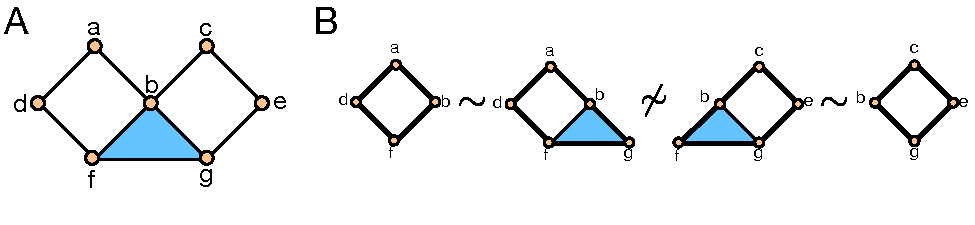
\includegraphics[]{./fig/background/homology_example.pdf}
\caption[Simplicial Homology]{(A) A simplicial complex defined on a set of 7 vertices, $S=\{a,\ldots,g\}$. The object has one connected component ($b_0=1$) and two holes ($b_1=2$). (B) Four cycles that can be defined on the complex. Cycles $z_1=\{(a,b)+(b,f)+(f,d)+(d,a)\}$ and $z_2=\{(a,b)+(b,g)+(g,f)+(d,f)+(d,a)\}$ are homologous, differing only by the cycle $c_1=\{(b,g)+(g,f)+(f,b)\}$ which is the itself the boundary of the closed triangle $(b,f,g)$. Likewise with cycles $z_3$ and $z_4$. The two sets of cycles are not homologous with each other, and there are therefore constitute two independent elements of the homology group $H_1(S)$. Note that the basis is not unique.}
\label{fig:bg:homology_example}
\end{figure}

\subsubsection{Constructing Complexes From Data}
\label{bg:tda:math:complexes}

Finally, we must consider how to construct a simplicial complex from a given point cloud $S$.\footnote{In fact, this step is arguably the most important step in applying a TDA pipeline.}
There are two common constructions we will describe: the \emph{\Cech\ complex} and the \emph{Vietoris-Rips complex}.
Both constructions involve a scale parameter $\epsilon$, and balls of radius $\epsilon$ placed at the center of each vertex in $S$.
Edges are drawn between vertices when balls overlap, that is, when $d(v_{a},v_{b})<2\epsilon$.
Where the two constructions differ is in how higher-dimensional simplices are filled in.

The \Cech\ complex consists of the set of simplices $\sigma$ with vertices $s_{1},\ldots,s_{k}\in S$ such that
\begin{equation}
\text{\Cech}(S, \epsilon) = \left\{ \sigma\in S \:|\: \displaystyle\cap_{i}^{} B(s_{i},\epsilon)\neq0 \right\}.
\end{equation}
That is, the simplex $\sigma_{(s_{x},\ldots,s_{z})}$ is present if the intersection of balls of radius $\epsilon$ centered on vertices $(s_{x},\ldots,s_{z}	)$ is nonempty.
The Vietoris-Rips complex, $VR(S,\epsilon)$, is defined as
\begin{equation}
\mathrm{VR}(S, \epsilon) = \{ \sigma\in S\:|\:\mathrm{diam}(\sigma) \leq 2\epsilon \}
\end{equation}
where $\mathrm{diam}(\sigma)=\{ \sup d(i,j) \:|\: i,j\in\sigma \}$.
In the Vietoris-Rips complex, a higher-dimensional simplex is filled in if every pairwise distance is less than $2\epsilon$.
The difference between the two constructions is shown in Figure~\ref{fig:bg:triangle_complexes}.
In general, $\text{\Cech}(S,\epsilon)\in VR(S,\epsilon)$.

The \Cech\ complex is theoretically preferable because it comes with a \emph{Nerve theorem}, which essentially states that the topology of the resulting complex will be equivalent to the topology of the union of balls used to create it.
However, the \Cech\ complex has drawbacks that prevent it from being widely applied to real data.
First, computing the intersection of arbitrary balls is an expensive operation.
While efficient algorithms exist in Euclidean space (the miniball algorithm \cite{Gartner:1999}), it is much more difficult in arbitrary metric spaces.
Furthermore, the \Cech\ construction explicitly requires an ambient space in which the data is embedded.
For data which comes in the form of a finite metric space, it may not be clear what is the ambient space.\footnote{This is indeed the case for the genomic data we consider: it is not immediately obvious what the intersection of three sequences defined over a finite alphabet should be. We discuss this further in Chapter~XX.}
In practice, the Vietoris-Rips complex is more widely applied, because it requires only the set of pairwise distances between each vertex and a scale parameter $\epsilon$.
The complex can be directly read off from the set of edges (known as the \emph{1-skeleton}), making it extremely fast to compute.

\begin{figure}
  \centering
  \subbottom[Three Points]{%
    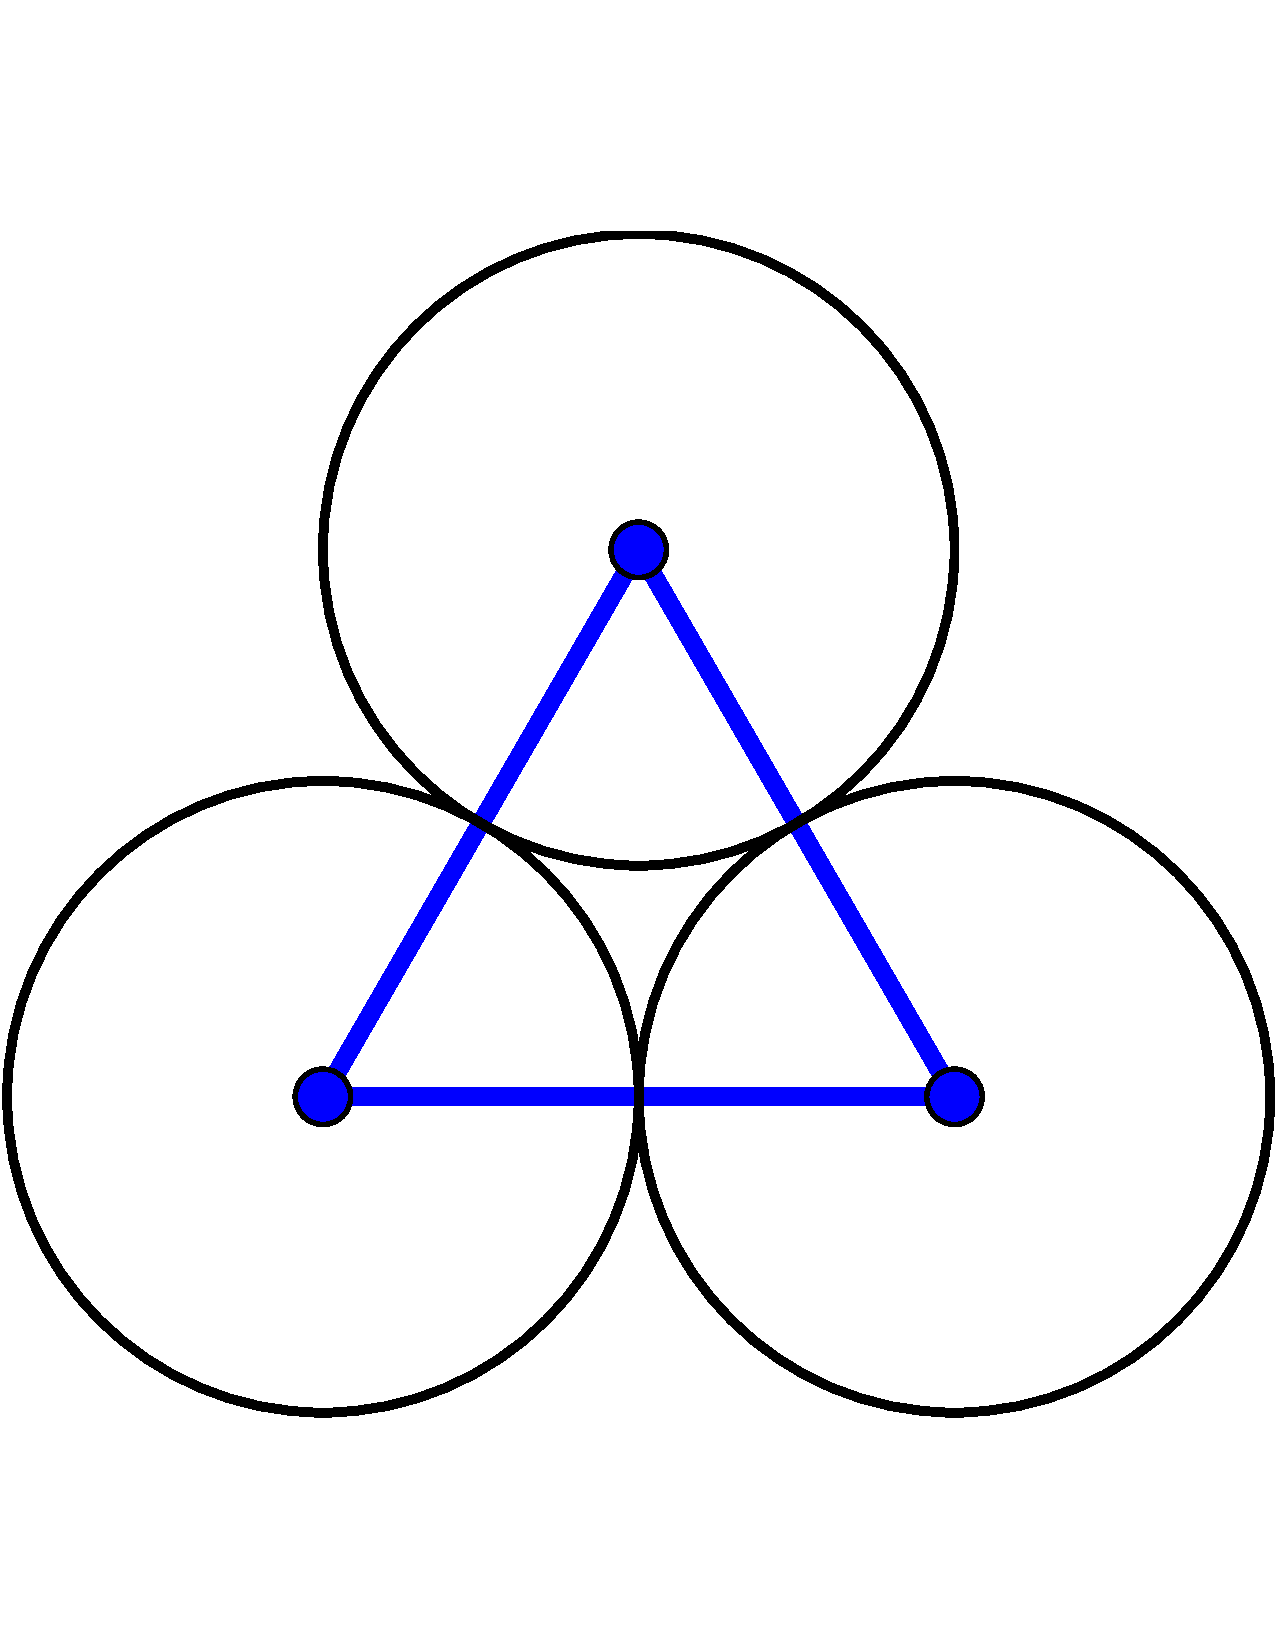
\includegraphics[width=0.25\linewidth]{fig/background/triangle_three_points.pdf}}
  \subbottom[Vietoris-Rips Complex]{%
    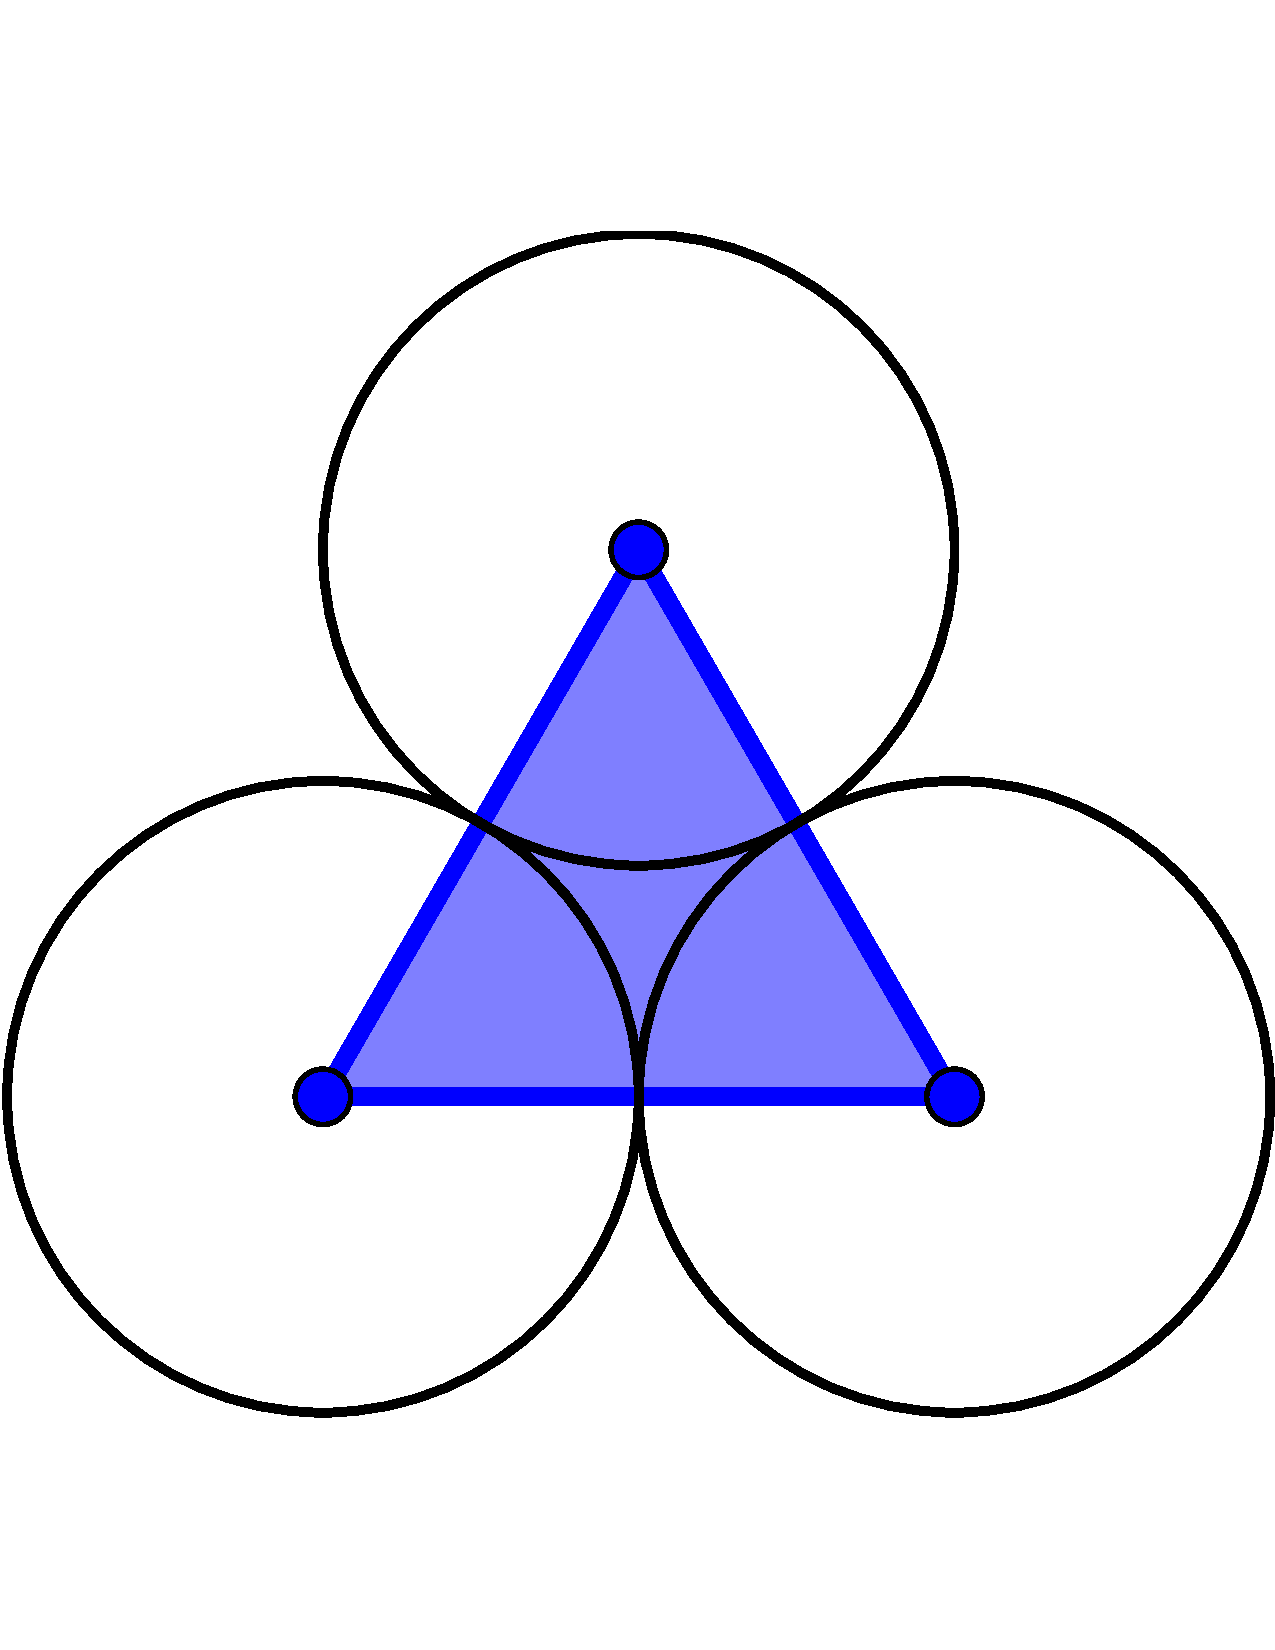
\includegraphics[width=0.25\linewidth]{fig/background/triangle_rips_complex.pdf}}
  \subbottom[\Cech\ Complex]{%
    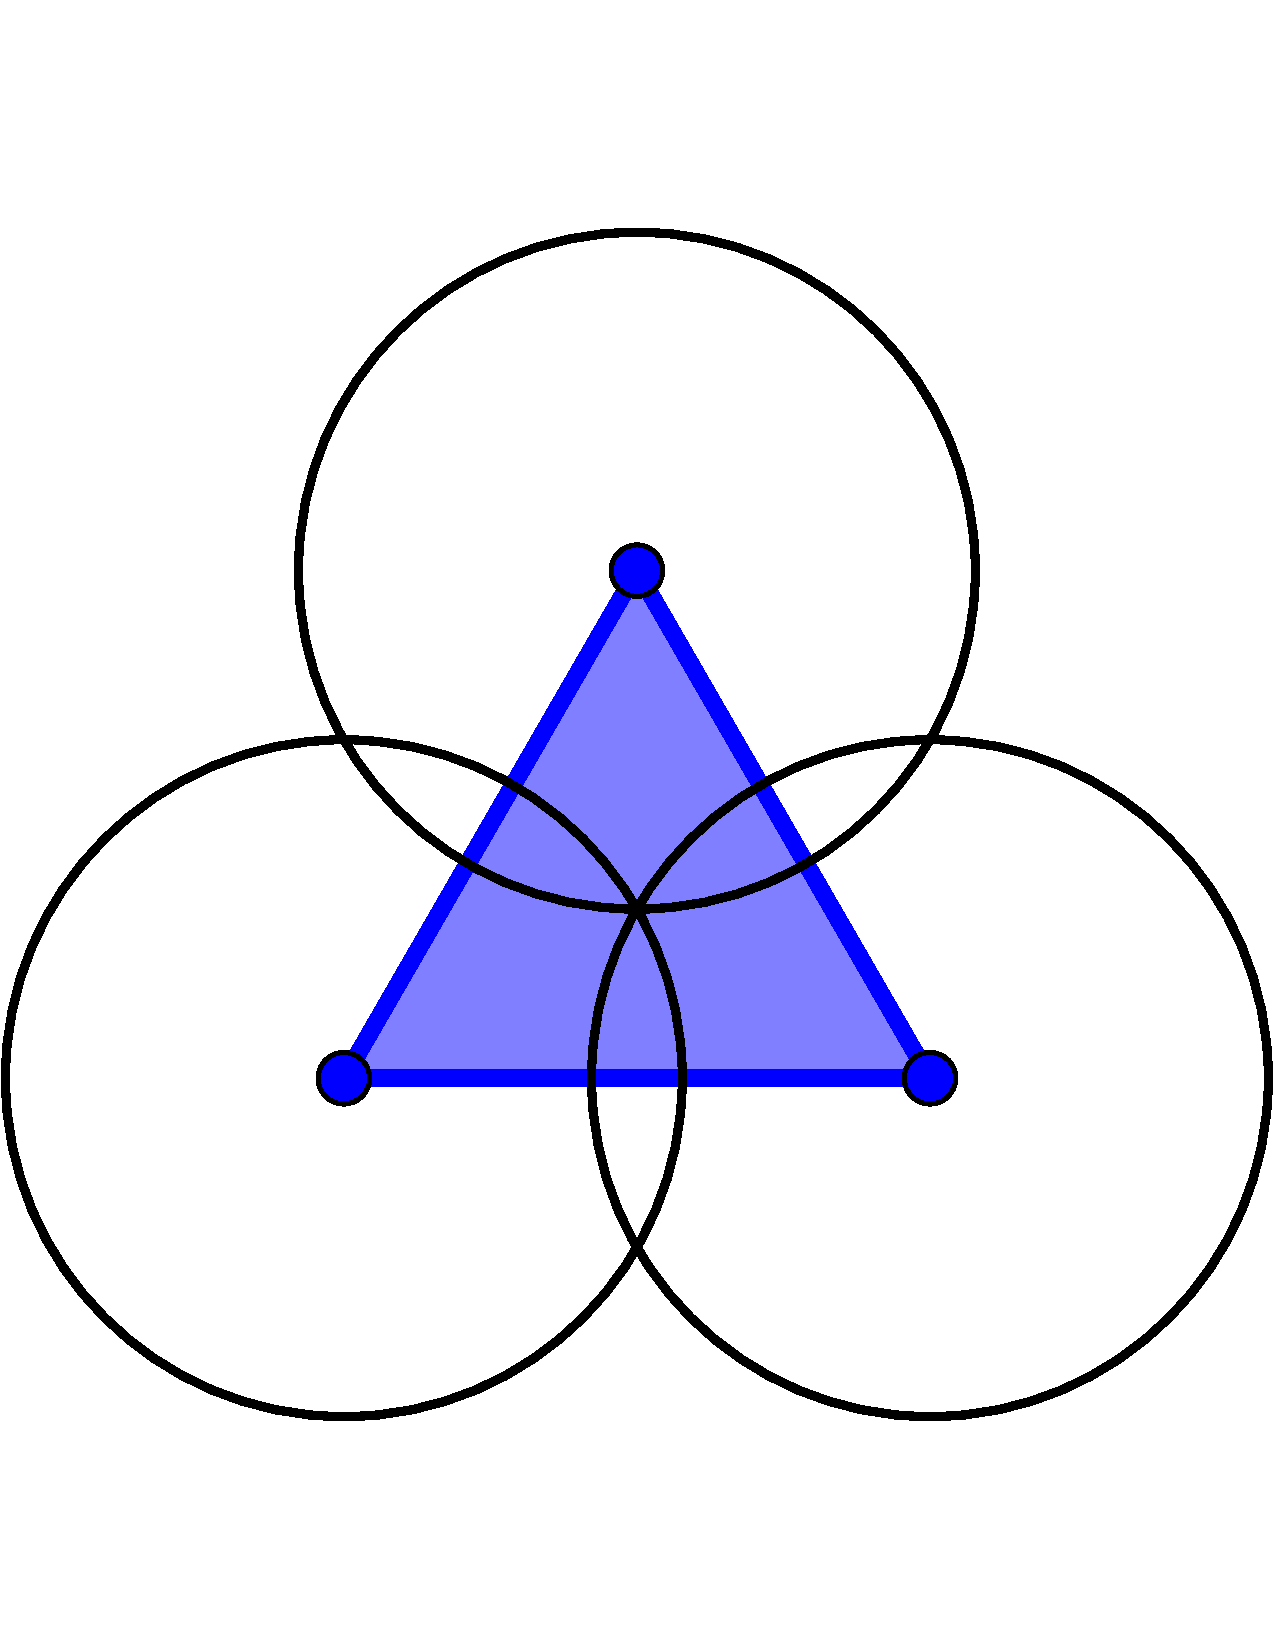
\includegraphics[width=0.25\linewidth]{fig/background/triangle_cech_complex.pdf}}
  \caption[Vietoris-Ripps and \Cech Complexes]{An example of the difference between Vietoris-Rips and \Cech\ complex on an equilateral triangle. Consider each point to be $1$ unit apart. In the Vietoris-Rips complex, the triangle is filled in when every pairwise edge is connected ($\epsilon=0.5$). In the \Cech\ complex, the triangle is only filled in when all three balls intersect ($\epsilon=0.577$).}
  \label{fig:bg:triangle_complexes}
\end{figure}
	
\subsection{Persistent Homology}
\label{bg:tda:ph}

Persistent homology is a tool developed under the umbrella of TDA that allows us to computationally study the shape of a point cloud across multiple scales simultaneously.
Shape is quantified in terms of topological invariants representing homology, as discussed in the previous section.
To understand why multiscale information might be of interest, consider the example in Figure~\ref{fig:bg:expanding_balls}.
The data is sparse and noisy, but, to the eye, immediately appears to consist of two circles joined at a point along their edges.
The two circles, however, are of a different radius.
In the Figure, we show Vietoris-Rips complexes constructed at different scale parameters on the data.
We observe that while some scale parameters are sufficient to resolve one or the other of the two circles, no single scale parameter is sufficient to simultaneously capture the two shapes.
Persistent homology solves this by providing a way to track the shape information across \emph{all} scale parameters.

Our object of study is the nested set of simplicial complexes, called a \emph{filtration}, that is produced by tuning the scale parameter up to some threshold.
At the smallest scale, $\epsilon=0$, the complex consists only of disconnected points.
As the scale parameter is increased, the topology of the complex changes -- clusters merge, holes and loops form, other holes and loops are filled -- until the complex is fully connected.
Each aspect of shape represents a topological invariant, and as the scale is changed, the birth and death of different invariants encoded as an interval $(b_i, d_i)$.

The shape information can be concisely summarized in a \emph{barcode diagram}.
The barcode diagram represents topological features as horizontal line segments, annotated with a birth-death interval, and a dimension.
The birth time is when a particular invariant first appears in the complex, and the death time is when the invariant is collapsed in the complex.
Shape information by dimension.
$H_0$ represents the number of connected components and is roughly equivalent to a hierarchical clustering of the data.
Higher dimensions represent loops ($H_1$), voids ($H_2$), and their generalizations in the data.
The number of bars at a particular scale will be the Betti number $b_n$ for that complex.
Taken together, the barcode diagram represents a complete and quantitative picture of the shape of the data.

The information can be equivalently represented as a persistence diagram, which is a scatter plot of invariants with birth time on the $x$ axis and death time on the $y$ axis.
The barcode diagram and persistence diagram for the two circles data is shown in Figure~\ref{fig:bg:expanding_balls_barcode}.
First, looking at $H_0$, we see that the data begins disconnected and becomes connected at around $\epsilon=24$.
Next, looking at $H_1$, we count eight loops across a range from \~5 to \~80.
Two of these loops persist for what appears to be an appreciable length of time.
We associate these two loops with the two circles that we identified qualitatively from the raw point cloud data.

The intuition behind persistent homology is exactly that: somehow the good or interesting features will be robust and persist over long scales.
In the barcode diagram, this corresponds to longer bars; in the persistence diagram, this corresponds to points sitting far from the diagonal.
Invariants that we observe persisting for only short scales are likely to be noise or other artifacts.\footnote{The obvious question of how to rigorously determine what makes a good interval is an open question that is currently being addressed by a number of different groups.We discuss this further in Section~\ref{bg:tda:ph:statistics}.}
And because a single scale is not capable of representing all features of the data, we examine all scales simultaneously.

\begin{figure}
\centering
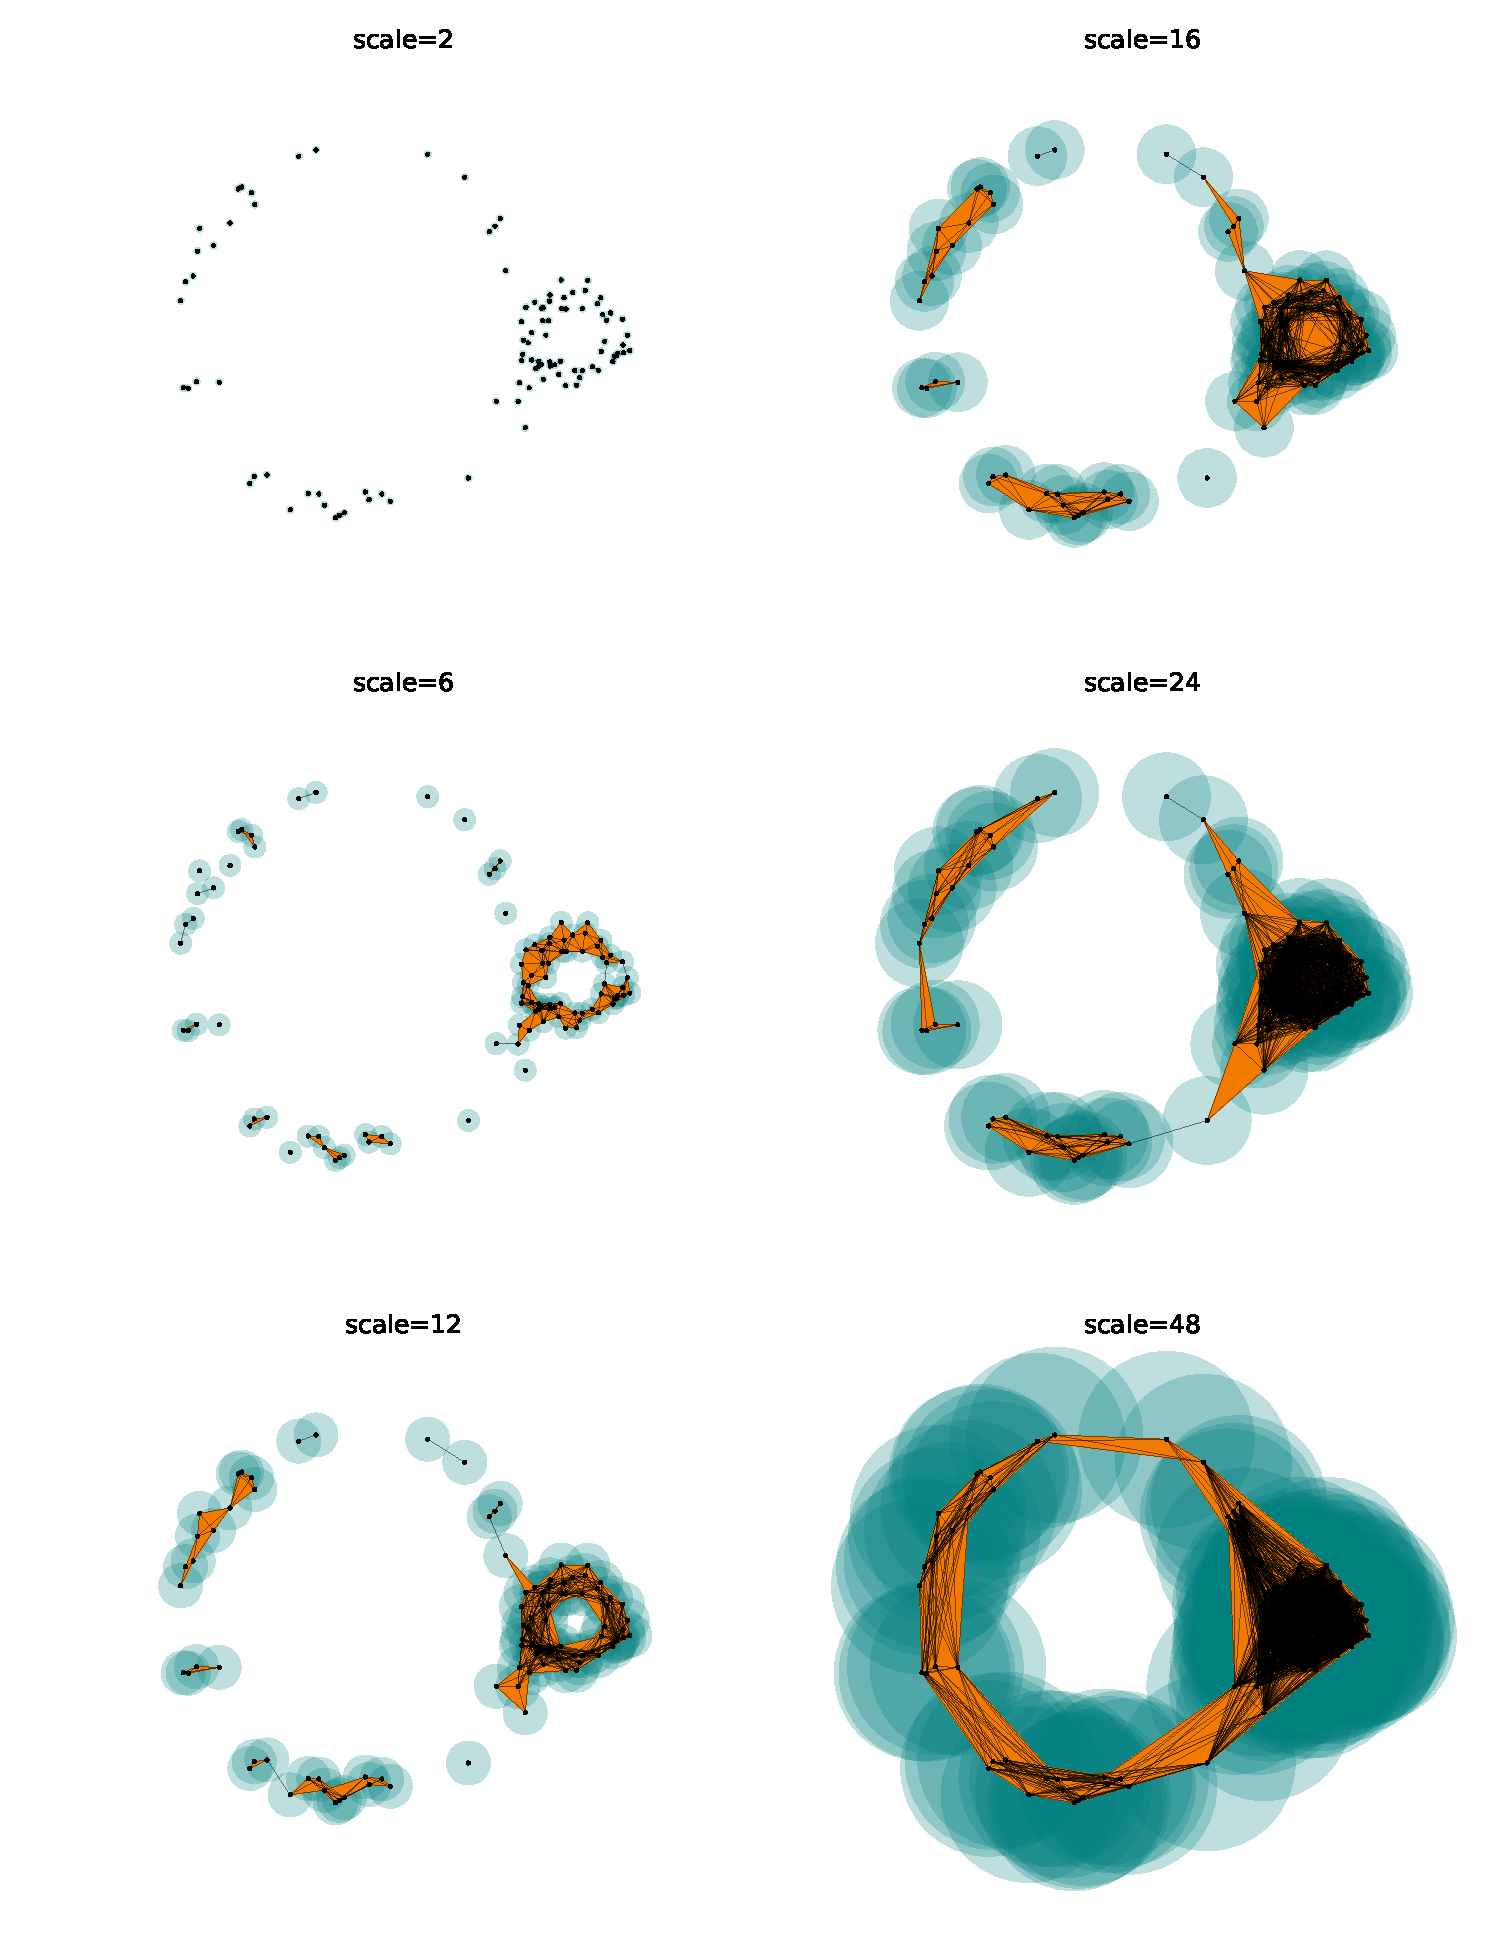
\includegraphics[width=.8\textwidth]{./fig/background/expanding_balls.pdf}
\caption[Multiscale Topological Structure]{An example of constructing a filtration. The nested series of complexes form a filtration. Persistent homology will compute and track the homology at each scale. Adapted from Lesnick.}
\label{fig:bg:expanding_balls}
\end{figure}

\begin{figure}
\centering
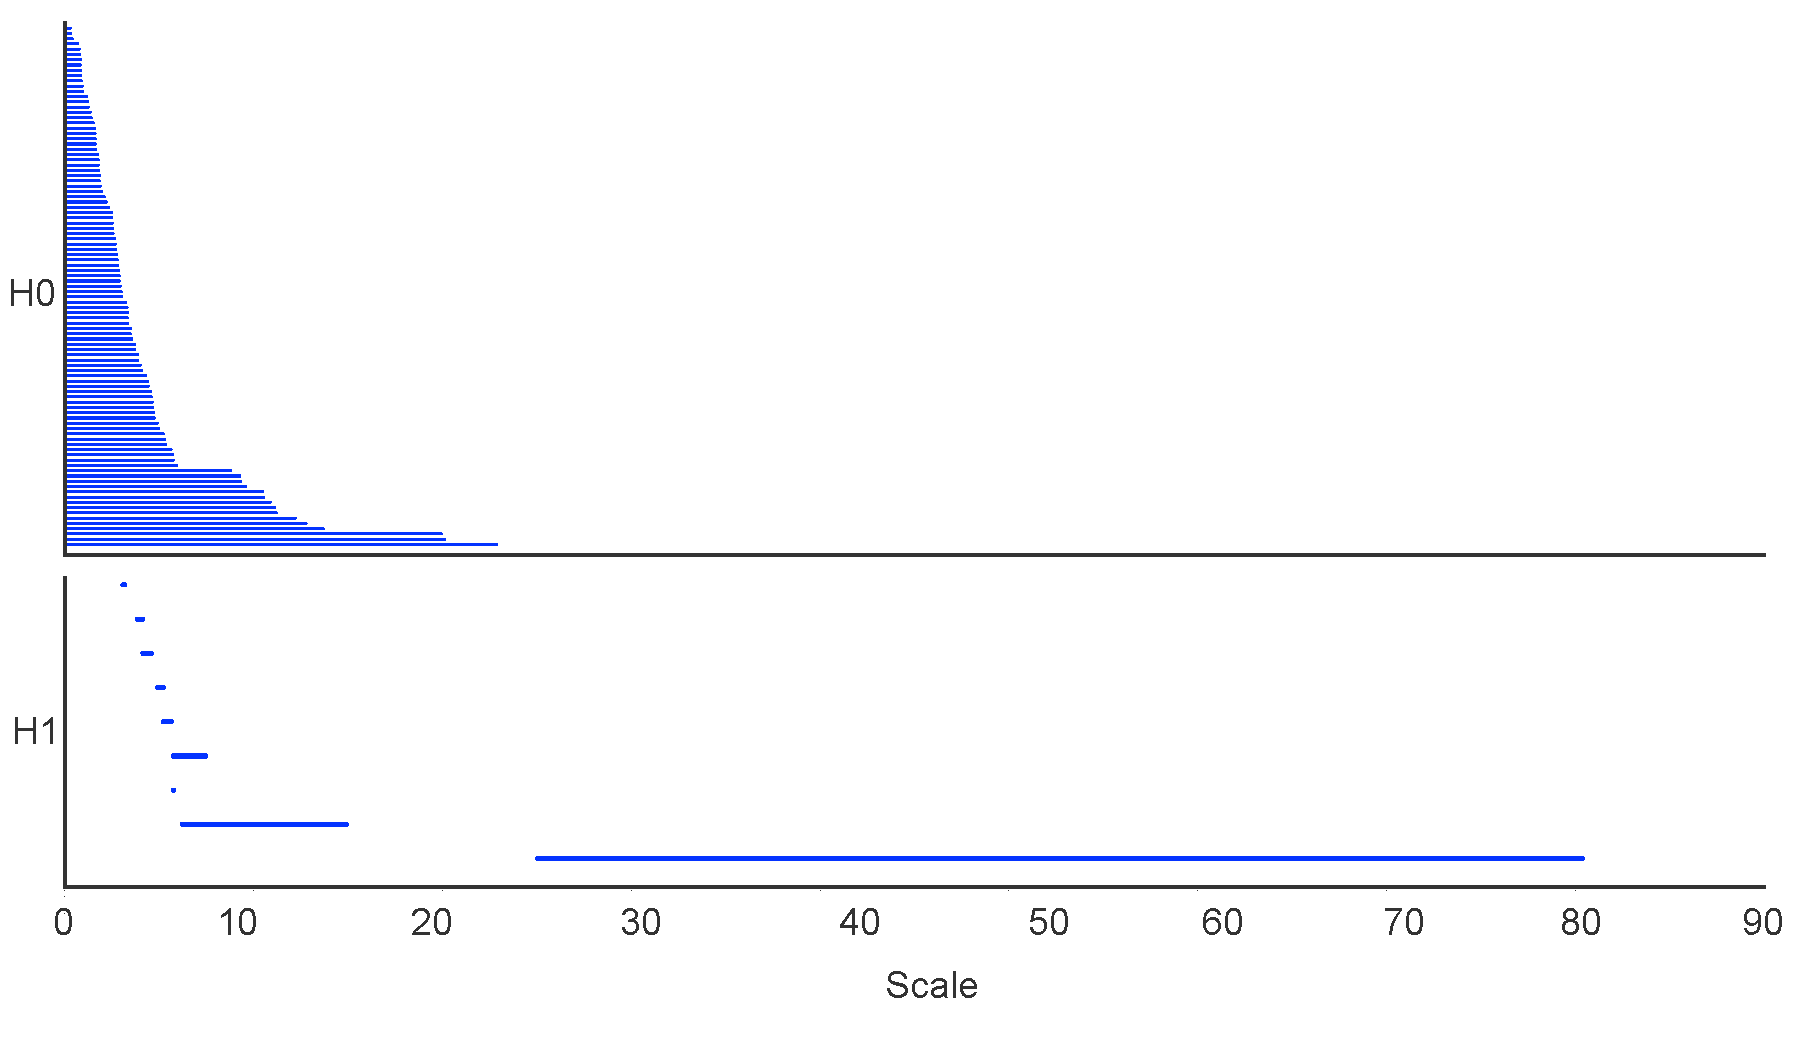
\includegraphics[width=.75\textwidth]{fig/background/expanding_balls_barcode.pdf}
\caption[Barcode Diagram for the Two Circles Example]{Barcode Diagram for the example in Figure~\ref{fig:bg:expanding_balls}. $H_0$ represents connectivity. $H_1$ represents the holes. Two holes are present at two different scales. Also some noise in the data.}
\label{fig:bg:expanding_balls_barcode}
\end{figure}

In fact, the persistence algorithm is more powerful than that, and can return not only the intervals associated with the invariants, but \emph{representative cycles} of each invariant.
The representative cycles correspond to the set of simplicies that surround an invariant, and can be used to determine which data points are somehow involved in a particular invariant.

To summarize, a complete description of the persistent homology pipeline is shown in Figure~\ref{fig:bg:persistence_pipeline}.
The pipeline is as follows:
A dataset, $S=(s_{1},\ldots,s_{N})$, is represented as a point cloud in a high-dimensional space (not necessarily Euclidean).
From the point cloud, a nested series of simplicial complexes, or a filtration, is constructed, parameterized by a filtration value $\epsilon$.
The filtration is represented as a list of simplices defined on the vertices of $S$, annotated with the $\epsilon$ at which the simplex appears.
Given a filtration, the persistence algorithm is used to compute homology groups.
The $0$-dimensional homology ($H_0$) represents a hierarchical clustering of the data.
Higher dimensional homology groups represent loops, holes, and higher dimensional voids in the data.
Each feature is annotated with an interval, representing the $\epsilon$ at which the feature appears and the $\epsilon$ at which the feature contracts in the filtration.
These filtration values are the \emph{birth} and \emph{death} times, respectively.

\begin{figure}[t]
\centering
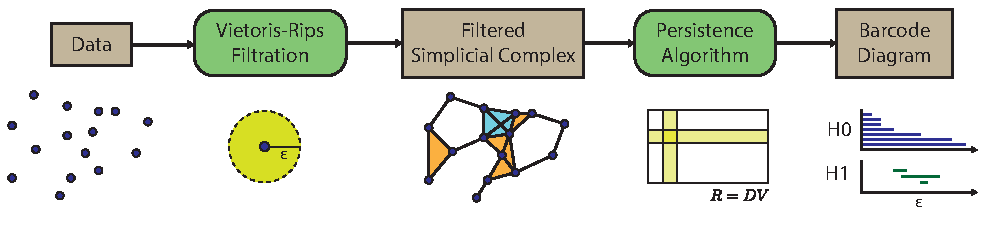
\includegraphics[]{./fig/background/persistence_pipeline.pdf}
\caption[The Persistence Pipeline]{The Persistence Pipeline.}
\label{fig:bg:persistence_pipeline}
\end{figure}

As primarily end-users of persistent homology, the details of the persistence algorithm are largely beyond the scope of this thesis.
Effectively, it involves manipulating the boundary matrix into a particular reduced form, from which each bar and representative cycle can be read off.
Several packages for computing persistent homology have been developed, including Javaplex \cite{Tausz:2011}, Dionysus \cite{Morozov:2012}, Perseus \cite{Nanda:2013}, Gudhi \cite{maria:hal-01108461}, and PHAT \cite{Bauer:PHAT:2015}.
Additionally, there is a TDA package for R which wraps functions from Dionysus and Gudhi in a user-friendly frontend \cite{Fasy:TDA:2015}.\footnote{In our work we have relied on a variety of these packages. For straight-forward construction of the barcode diagram, we find the R package TDA easiest to use. If one needs to directly build and manipulate filtered simplicial complexes, Dionysus has convenient Python bindings. For large datasets, PHAT and it's parallel implementation DIPHA \cite{Bauer:DIPHA:2015,Bauer:2014gd} are recommended.}

\subsubsection{Stability of the Persistence Algorithm}
\label{bg:tda:ph:stability}

While not strictly necessary in this thesis, the stability result is important 

While not directly utilized in this thesis, the statement of stability is important to include for
While not directly utilized in this thesis, the statement is important to include.
The stability result establishes that small perturbations in the data will produce only small changes in the the persistence diagram.
The stability result is 


The result of \citet{Chazal:2009wc} states that the bottleneck distance between $B$ and $B'$ is bounded by the Gromov-Hausdorff distance between the finite metric spaces embedded in $A$ and $B$.

An important aspect of peristent homology is stability.
Stability refers to how the output of persistent homology will change when the original data is perturbed, for example due to noise or sampling.
Will the existing bars change?
Will new homology classes be formed?
We would like the output of persistent homology to be stable under these perturbations.
In general, our question is if I have some perturbation that takes my data from $D\rightarrow D'$, what can I say about the subsequent change in barcodes $B\rightarrow B'$?
In general, if I have data $D$ that is perturbed to new data $D'$, how will change
Luckily, there is a result that bounds changes in the diagram, due to Chazal and coauthors \citep{Chazal:2009wc}.
After a few definitions, we state the stability theorem.

\begin{defn}
\label{defn:gromovhausdorff}
The \emph{Gromov-Hausdorff distance} measures how far two spaces are from being isometric.
It measures the longest distance from a point in one set to the closest point in another set within a metric space.
\begin{equation}
d_{GH}(X,Y)=\inf_{f,s} d_H(X,Y)
\end{equation}
\end{defn}

Next, we consider how to define the distance between two persistance diagrams.
To do so, we first need the concept of a \emph{matching}.
For two persistence diagrams $A$ and $B$, a matching is a mapping from intervals in $A$ to intervals in $B$, where we allow points to match to the diagonal to account for cases with unequal number of points.
For each matched pair of intervals $(a,b)$, we define the $L_{\infty}$ distance as

\begin{equation}
d_{\infty}(a,b) = \max\{ |a_{x}-b_{x}|, |a_{y}-b_{y}| \}.
\end{equation}

\begin{defn}
\label{defn:bottleneck}
The \emph{bottleneck cost} of a matching between two diagrams is the maximum $L_{\infty}$ for all matched points. The \emph{bottleneck distance} is defined to be the minimal bottleneck cost across all matchings. The matching with minimal bottleneck cost is the \emph{bottleneck matching}.
\begin{equation}
d_{B}(A,B) = \inf_{n:A\rightarrow B} \sup_{x\in X} ||x-\eta(x)||_{\infty}
\end{equation}
\end{defn}

\begin{thm}
\label{thm:stability}
The stability theorem.
\begin{equation}
d_{B}(H_{K}(X),H_{K}(Y)) \leq d_{GH}(X,Y)
\end{equation}
\end{thm}

\subsubsection{Statistical Persistent Homology}
\label{bg:tda:ph:statistics}

%% write this section today (just briefly)

Statistical persistent homology addresses two questions: (1) how to distinguish 

In persistent homology, the intuition is developed that long intervals are to be interpreted as large-scale, robust, or in some sense real geometric features of the data, while short intervals are more likely to correspond to noise or random effects due to incomplete sampling.

However, this leaves open the question of determining how long a bar must be to be considered significant.
How short is short, and how will noisy sampling effect the observed diagram?
When can a long interval be interprested as a real feature?
In general, one would like to be able to develop statistics from the barcode diagram and assign measures of confidence to our estimates.
How to use encode the barcode diagram in such a way that statistics can be used.

Substantial recent work in the TDA community has focused on these questions in order to develop statistical foundations for persistent homology.
We give here a brief flavor of some of these ideas and their relation to our own work.

There are two main approaches to statistical peristent homology.
The first computes functional summaries of the barcode diagram, which can then be used in downstream in a machine learning setting.
In the first, functional summaries of the persistence diagram are computed.
These functional summaries can be fit to known distributions and used to make inferences.
In the second, probability measures on the space of persistence diagrams are directly computed.
These approaches require the space of persistence diagrams to satisfy certain properties, such as being a Polish space.
A Polish space has a well defined notion of mean and variance.

\begin{itemize}
\item Probability measures on the space of persistence diagrams
\item Functional summaries of the persistence diagram
\item Confidence intervals on the persistence diagram
\item Statisical inference using persistence diagrams
\end{itemize}

Fasy and coauthors have developed ways of generating confidence intervals for persistence diagrams \citep{Fasy:2014}.
Based on some information about density, they can put a line off the diagonal below which points are to be considered noise (see example).
Bubenik has developed the language of persistence landscapes \cite{Bubenik:2007ux,Bubenik2015:um}.  
Several authors have examined the space of persistence diagrams as a Polish space, with notions of mean and variance.
XXX et al have used the bootstrap to get estimates of the diagram robustness.

Also see the work of Turner \cite{Turner:2012wb}, Mileyko \cite{Mileyko:2011jm}, and Mukherjee.

\subsubsection{Multidimensional Persistence}
\label{bg:tda:ph:multid}

First laid out in \cite{Carlsson:2009b}.
More work in \cite{Lesnick:2012uv}.
Filtrations along different dimensions; how to relate?.
Prototypical example: density and distance.

Our case is going to be slightly different.
We will consider a set of points annotated with different metrics that we can put on it which will induce different homologies.
Then we will see what happens we interpolate between those different metrics.
\kje{[Discuss with Michael.]}

\subsection{Mapper}
\label{bg:tda:mapper}

% insert Mapper description here.
Mapper sits within the large universe of dimensionality reduction algorithms for exploratory data analysis.
Mapper allows for qualitative analysis of high-dimensional data through direct visualization.
In this sense it belongs within the larger category of dimensionality reduction techniques such as multidimensional scaling (MDS) and their nonlinear extensions, including Isomap and t-SNE.

Mapper has the following advantages:

(1) Coordinate free
(2) Invariance to deformation - robustness to noise
(3) Compressed representation - ability to handle large datasets.

The \emph{Mapper} algorithm was developed by Gurjeet Singh and Gunnar Carlsson in \cite{Singh:2007ve}.
Further exposition can be found in \cite{Lum:2013cz}.
Mapper was first applied to problems in RNA folding in \cite{Bowman:2008esa} and breast cancer subtype identification in \cite{Nicolau:2011}.

Steps:
(1) Project using filter function.
(2) Create overlapping bins
(3) Cluster in the projected space.
(3) Connect pairs of bins with shared points

Our use of the Mapper algorithm will be relatively minimal.
We use it as a means to visualize our sequence data in such a awy
In our work we use the commercial implementation of Mapper developed by Ayasdi \cite{AyasdiIris:2015}.
An open-source implementation of Mapper is available in the Python Mapper package \cite{Mullner:2013}.

\begin{figure}
\begin{tikzpicture}[node/.style={minimum height=.8cm,minimum width=2cm,draw}]
\draw (0,0) node[node, align=center] (dr) {Dimensionality\\Reduction};
\draw (3,1) node[node] (linear) {Linear};
\draw (3,-1) node[node] (nonlinear) {Nonlinear};
\draw (6,1) node[node] (pca) {PCA};
\draw (6, -.5) node[node] (geometry) {Geometry};
\draw (6, -1.5) node[node] (topology) {Topology};
\draw (9, -.5) node[node,align=left] (manifold_learning) {Manifold\\Learning};
\draw (9, -1.5) node[node] (mapper) {Mapper};
\draw (12, -.5) node[node,align=center] (mds) {MDS\\PCA\\Isomap};


\myline{dr}{linear};
\myline{dr}{nonlinear};
\draw[-latex] (linear) -- (pca);
\myline{nonlinear}{geometry};
\myline{nonlinear}{topology};
\draw[-latex] (topology) -- (mapper);
\draw[-latex] (geometry) -- (manifold_learning);
\draw[-latex] (manifold_learning) -- (mds);

\end{tikzpicture}
\caption[Dimensionality Reduction for EDA]{Dimensionality Reduction for EDA}
\label{fig:bg:eda}
\end{figure}

\section{Applying TDA to Molecular Sequence Data}
\label{bg:top4bio}

Aligned molecular sequence data can be naturally viewed as a point cloud in a high-dimensional space, which we loosely call \emph{sequence space}.
The particular structure of sequence space will be determined by the length, $L$, of the aligned sequences, and the alphabet, $Q$, over which the sequences are defined.
A typical sequence alphabet will be either nucleotides or amino acids.
The dimension of the space is determined by $L$.
Sequence space will therefore consist of the $||Q||^L$ possible sequences.
Together with any of the standard genetic distance measures, this forms a finite metric space.

The process of evolution can be seen as an exploration of sequence space.
An individual genotype can be assigned a fitness, $w$, which will describe the probability of reproductive success in a particular environment.
Clonal evolution is the process of smoothly moving through sequence space, while reticulate evolution is the process of making discontinuous jumps through the space.

Our data generally consists of a subset of points sampled from sequence space.
These points reflect a particular evolutionary history.
As more data is acquired, areas of sequence space will become more densely sampled and the ability to reconstruct that evolutionary history will become more feasible.
Given molecular sequence data, our program is to (1) encode the data as a finite metric space, (2) use tools from TDA to characterize the topology of the data, and (3) interpret the topology in an evolutionary context.
In particular, we apply persistent homology, and read phylogenetic information contained in the dataset off the resulting barcode diagram.
We make two preliminary remarks before considering a more complete example.

\subsection{Topology of Tree-like Metrics}
\label{bg:top4bio:treemetrics}

An important foundational point was demonstrated by G. Carlsson in \cite{Chan:2013}.
Recall that tree-like data will have an additive metric space, as described in Section~\ref{bg:bio:phylo:additivity}.
In \cite{Chan:2013}, it was proven that for additive metric spaces, the Vietoris-Rips filtration of the data will consist of a nested set of acyclic complexes.
Consequently, the persistent homology of additive data will have nontrivial topology only in dimension zero.
Furthermore, while noise in the data an introduce small deviations from additivity, the theorem puts bounds on the size of the topological features that can arise in this manner.
These bounds rely on the Gromov-Hausdorff stability conditions described in Section~\ref{bg:tda:ph:stability}.

On the other hand, if the evolutionary history includes reticulate events that cannot be represented as a tree, these events will be captured as non-trivial higher dimensional homology in the barcode diagram, an idea which we develop below.
This theorem provides an important positive control in using TDA to characterize reticulate evolution.

\subsection{The Fundamental Unit of Reticulation}
\label{bg:top4bio:fundamental_unit}

In population genetics, there is a simple test for the presence of reticulate evolution in sequence data called the \emph{four-gamete test} \cite{Hudson:1985}.
The test assumes only an infinite-sites model, which states that for a sufficiently long genome, a particular residue can only ever undergo a single mutation.
Put another way, there is no multiple-mutation or back mutation.
The infinite-sites model has three consequences: first, one need only consider segregating sites, or nucleotide positions that have undergone a mutation.
Second, because a given position can mutate only once, it is sufficient to represent sequences as binary strings, where a $0$ indicates the unmutated state and $1$ the mutated state.
Third, for a given position we can arbitrarily assign the unmutated and mutated states.
The infinite-sites model is considered a reasonably good model for long genomes.

The four-gamete test identifies reticulate evolution by looking at pairs of segregating sites.
Given biallelic data, there are four possible haplotype patterns, or states, for a pair of segregating sites: $00$, $10$, $01$, or $11$.\footnote{These sites need not be adjacent.}
The statement of the four gamete test is this: in any given dataset, the simultaneous presence of all four haplotype states in any pair of segregating sites is incompatible with strictly clonal evolution, and indicates reticulate evolution.
To see this, assume state $00$ as the ancestor to states $10$ and $01$, which arise from two independent mutations.
Because of the no multipe-mutation assumption, it is not possible for either of these two states to then independently mutate into state $11$.
The only way for state $11$ to arise is via a reticulate event that brings together the left site from state $10$ and the right site from $01$.\footnote{It is entirely possible for the reticulate event to have had a reversed pattern of ancestry, in which case the reticulation would result in a state $00$ and would not be detectable from the sequence data.}
This process is illustrated in Figure~XXA.

Under a Hamming metric, the distance matrix for the set of four sequences $s_1=00$, $s_2=10$, $s_3=01$, and $s_4=11$ is
\begin{equation}
d = 
\begin{pmatrix}
0 & 1 & 1 & 2 \\
1 & 0 & 2 & 1 \\
1 & 2 & 0 & 1 \\
2 & 1 & 1 & 2 \\
\end{pmatrix}
\end{equation}
The Vietoris-Rips filtration of this space is shown in Figure~\ref{fig:bg:four_gamete_test}C.
At $\epsilon=0$ the four sequences are disconnected.
At $\epsilon=1$, four edges are drawn, forming a loop.
At $\epsilon=2$, the space is completely connected and the loop is killed.
Persistent homology captures the presence of this loop as an $H_1$ feature in the interval $[1,2)$ (Figure~\ref{fig:bg:four_gamete_test}D).
In this way, the reticulate event is associated with the presence of a nonzero $H_1$ bar.

We consider this example to be the minimal, or fundamental, unit of reticulation.
All more complicated patterns of reticulation can be seen as extensions of this example.

\begin{figure}
\centering
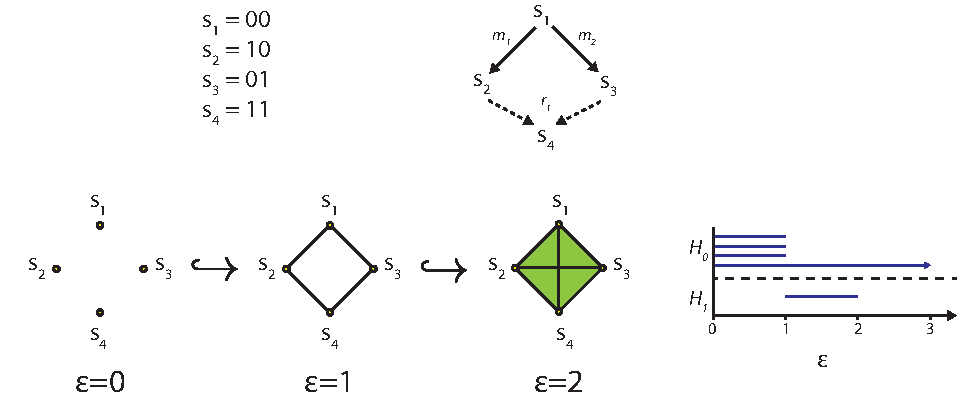
\includegraphics[width=\textwidth]{./fig/background/four_gamete_test.pdf}
\caption[Fundamental Unit of Reticulation]{The Fundamental Unit of Reticulation. (A) A set of four sequences. (B) An evolutionary genealogy including two mutations ($m_1$ and $m_2$) and a single reticulation ($r_1$). (C) Vietoris-Rips Filtration. (D) Barcode Diagram.}
\label{fig:bg:four_gamete_test}
\end{figure}

\subsection{A Complete Example}
\label{bg:top4bio:full_example}

We illustrate a complete example of how TDA can capture horizontal evolution from complex populaton data in Figure~\ref{fig:bg:tda_on_sequence_data}.
Consider the reticulate phylogeny (Figure~\ref{fig:bg:tda_on_sequence_data}A): five genetic sequences sampled today (yellow circles) originate from a single common ancestor due to clonal evolution (solid blue lines tracing parent to offspring) and reticulate evolution (dotted red lines).
In Figure~\ref{fig:bg:tda_on_sequence_data}B, these five samples are placed in the context of a larger dataset, where the data has been projected onto the plane using PCA.
Persistent homology is then applied to this larger sample.
In Figure~\ref{fig:bg:tda_on_sequence_data}C we demonstrate the construction of a filtered simplicial complex, showing how the connectivity changes as the scale parameter $\epsilon$ is increased.
Finally, in Figure~\ref{fig:bg:tda_on_sequence_data}D we see the resulting barcode diagram.
Using $H_0$ we can track the number of strains or subclades that persist, roughly corresponding to the tree-like component of the data.
The $H_1$ bar near spanning roughly $\epsilon=0.13$ to $\epsilon=0.16$ identifies the presence of a reticulate event. involving the five higlighted sequences.
The scale over which this bar persists represents the amount of evolutionary time separating the parents and the reticulate offspring.
Additionally, the persistence algorithm will return a generating basis for a particular homology group, which we can use to identify the particular mixtures of sequences involved a reticulation.
In this way, we can analyze both the scale and frequency of reticulation in genomic data sets.

We summarize the connection between genomic data and TDA in Table~\ref{table:dictionary}.

\begin{table}
\centering
\caption{Dictionary connecting algebraic topology and evolutionary biology}
\small
\rowcolors{2}{gray!25}{white}
\setlength{\aboverulesep}{0pt}
\setlength{\belowrulesep}{0pt}
\setlength{\extrarowheight}{.75ex}
\begin{tabularx}{\textwidth}{XX}
\toprule\rowcolor{gray!50}
Algebraic Topology                                         & Evolutionary Biology \\
\midrule
Filtration value $\epsilon$                                & Genetic distance (evolutionary scale) \\
0-dimensional Betti number at filtration value $\epsilon$  & Number of clusters at scale $\epsilon$ \\
Generators of 0-D homology                                 & A representative element of the cluster \\
Hierarchical relationship among generators of 0-D homology & Hierarchical clustering \\
1-D Betti number                                           & Lower bound on number of reticulate events \\
Generators of 1-D Homology                                 & Reticulate events \\
Generators of 2-D Homology                                 & Complex horizontal genomic exchange \\
Non-zero high-dimensional homology (“topological obstruction to phylogeny”) & No treelike phylogenetic representation exists \\
Number of higher-dimensional generators over a time interval (“irreducible cycle rate”) & Lower bound on recombination/reassortment rate \\
\bottomrule
\end{tabularx}
\label{table:dictionary}
\end{table}

\begin{figure}
\centering
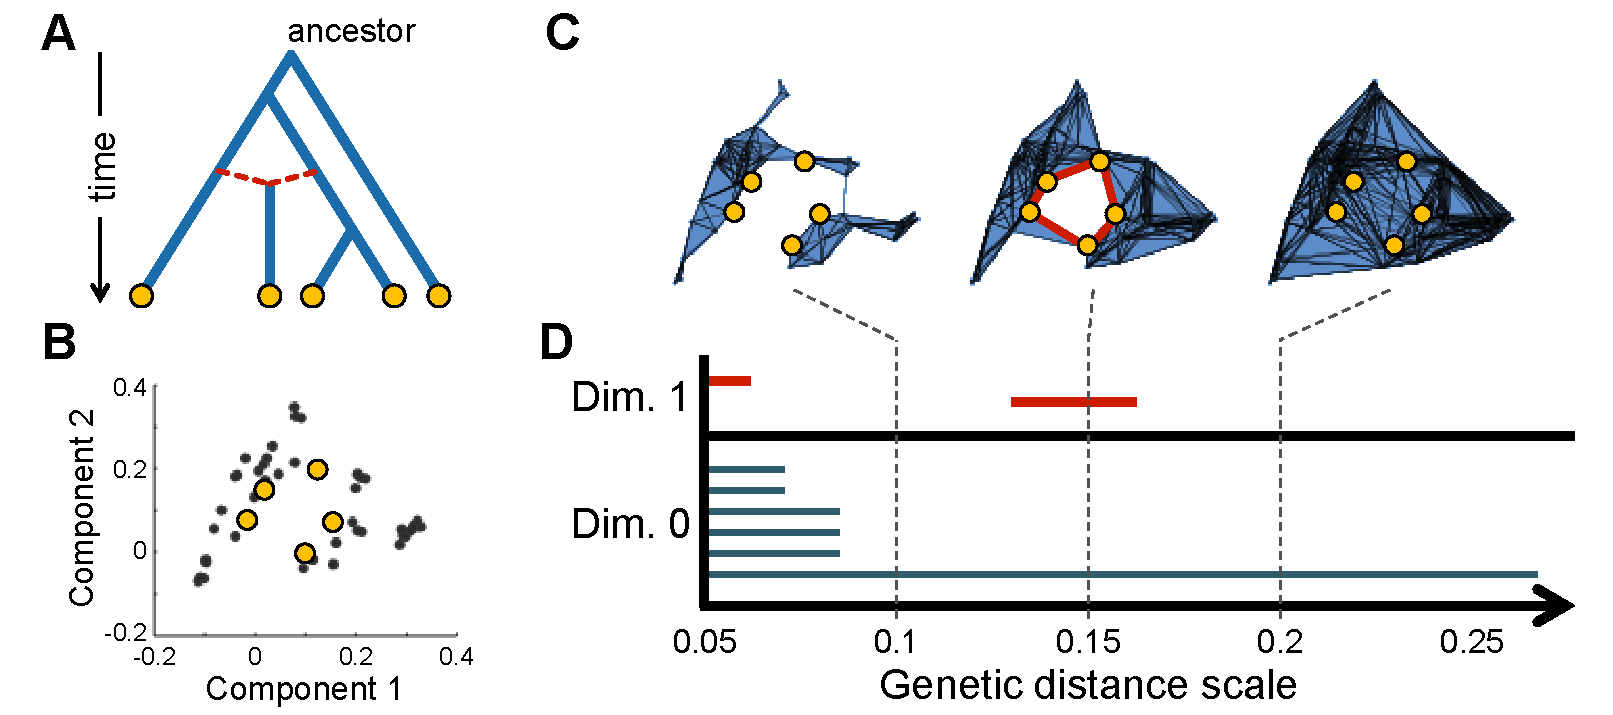
\includegraphics[width=\textwidth]{./fig/tda_on_sequencedata.pdf}
\caption[Applying TDA to Molecular Sequence Data]{Applying persistent homology to genomic data. (A) An evolutionary genealogy including reticulation. (B) Data projected into 2-dimensions. (C) Construction of a filtered simplicial complex. (D) The resulting multiscale barcode diagram.}
\label{fig:bg:tda_on_sequence_data}
\end{figure}

\subsection{The Space of Trees, Revisited}
\label{bg:top4bio:tree_space}

In Section~\ref{bg:bio:phylo:space}, tree space was introduced as an abstract construction to systematically represent the set of all possible binary trees.
Further, we have shown that additive metrics can be represented as binary trees in tree space.
Because real sequence data will very rarely satisfy the additivity condition, one possible interpretation of phylogenetic reconstruction is of finding the best projection onto tree space for arbitrary data.

The complete space of finite metrics on $L$ vertices is $(\mathbb{R}^{\geq 0})^{\binom{L}{2}}$
Tree space will be a set of $(2L-5)!!$ subspaces of dimension $\mathbb{R}^{L-3}$.

The program we propose can be understood as an extension of the tree space framework.
Rather than attempt to characterize arbitrary data as a projection onto tree space, we will use methods of TDA to compute topological invariants.
The intuition we develop is that as we move off of tree space, there is no additive tree that can represent the data.
We would like a topological measure of deviation from addivity.
Luckily, from the theorem due to Carlsson, we know we can use homology as this measure.
Higher homology will vanish for additive, tree-like, metrics.
The hypothesis is that the further the data lives from tree space, the larger or more these invariants will be.
The deviations from additivity are telling us something about the scale and frequency of reticulate evolution in the dataset.
Our updated picture looks as Figure~\ref{fig:bg:tree_space_revisited}.
We have tree space, however it is now e
Tree space is a subspace of 

Note that this is an abstract construction and for data sets with an appreciable number of leaf nodes it will be difficult to directly visualize their position.
Our hope is that the topological tools we develop here are sensitive enough to capture these deviations in interpretable ways.

Finally, we note that at the outset of this work, an ambitious goal was set to provide a complete characterization of the space of finite metrics in terms of their topological invariants as measured by persistent homology.
While some interesting work has explored the combinatorial structure of the space of metrics on low numbers of points (see \cite{Sturmfels:2004vc}), it does not appear feasible in general to provide a complete decomposition.

\begin{figure}
\centering
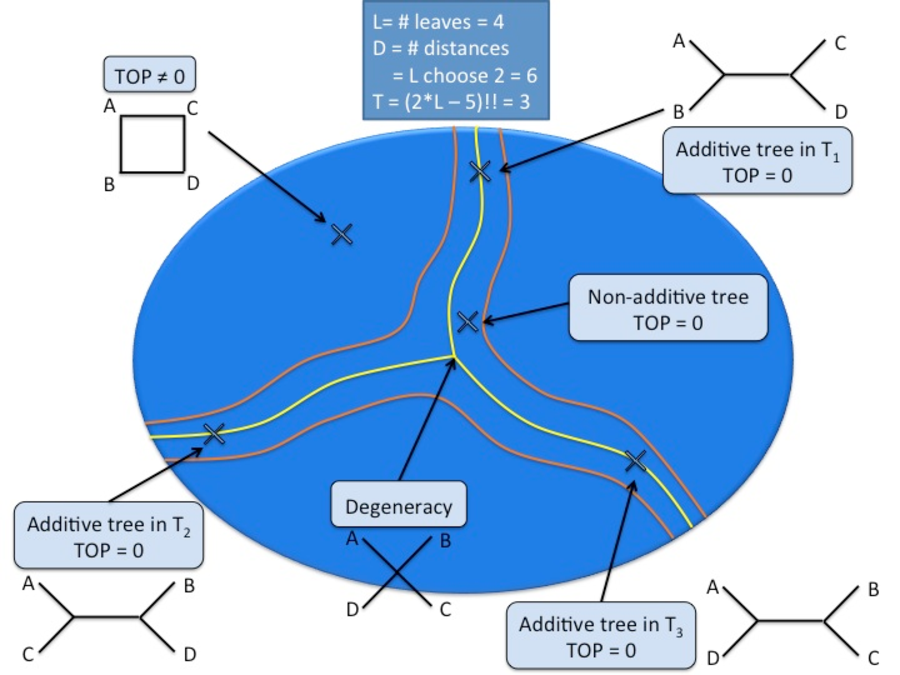
\includegraphics[]{./fig/background/tree_space_revisited.pdf}
\caption[Tree Space Revisited]{In light of reticulate evolution, our domain of interest can be expanded from the original tree space construction. We are now interested in data that lies off of tree space. We will use topology and TDA to characterize the deviations from additivity.}
\label{fig:bg:tree_space_revisited}
\end{figure}